\section{Phân tích hiệu quả tương tác của bài đăng trên mạng xã hội facebook}
\subsection{Giới thiệu chung}
Trong thời đại kỹ thuật số, mạng xã hội đã trở thành một phần không thể thiếu của cuộc sống hàng ngày. Các nền tảng như Facebook, Twitter, Instagram, LinkedIn, và TikTok không chỉ là nơi để kết nối bạn bè mà còn là môi trường quan trọng để doanh nghiệp tương tác với khách hàng, chính trị gia tiếp cận cử tri, và các nhà hoạt động xã hội lan tỏa thông điệp của họ.

\subsection{Phát biểu bài toán}
\textbf{Tại sao phân tích tương tác trên mạng xã hội lại quan trọng?}

Phân tích tương tác trên mạng xã hội là quá trình thu thập, phân tích và diễn giải các dữ liệu về hành vi của người dùng, bao gồm các lượt thích, chia sẻ, bình luận, và các loại tương tác khác. Bài toán đặt ra là cần hiểu rõ tầm quan trọng của việc phân tích này để từ đó tối ưu hóa các chiến lược truyền thông, tiếp thị, và xây dựng thương hiệu.

\subsection*{Các khía cạnh của bài toán}
\begin{itemize}
    \item \textbf{Đo lường hiệu quả chiến lược tiếp thị:} 
    Phân tích tương tác giúp xác định những chiến dịch tiếp thị nào đang hoạt động hiệu quả và đâu là những điểm cần cải thiện. Bằng cách theo dõi các chỉ số như lượt thích, chia sẻ, và bình luận, các nhà tiếp thị có thể điều chỉnh chiến lược để tăng tương tác và thu hút khách hàng.

    \item \textbf{Xây dựng thương hiệu và tăng cường sự hiện diện:} 
    Tương tác cao thường liên quan đến nhận diện thương hiệu mạnh và sự trung thành của khách hàng. Phân tích tương tác giúp xác định những nội dung hoặc chủ đề nào có sức hút đối với người theo dõi, từ đó thúc đẩy việc tạo ra nội dung phù hợp hơn.

    \item \textbf{Hiểu rõ hành vi người dùng:} 
    Phân tích tương tác cung cấp cái nhìn sâu sắc về sở thích và hành vi của người dùng. Hiểu được những gì người dùng thích hoặc không thích có thể giúp doanh nghiệp tạo ra sản phẩm, dịch vụ hoặc nội dung phù hợp hơn với nhu cầu của họ.

    \item \textbf{Phát hiện xu hướng và cơ hội:} 
    Phân tích tương tác cho phép doanh nghiệp và tổ chức phát hiện sớm các xu hướng mới nổi, từ đó tận dụng cơ hội để dẫn đầu thị trường hoặc cộng đồng của mình.

    \item \textbf{Quản lý khủng hoảng:} 
    Khi có khủng hoảng hoặc phản hồi tiêu cực trên mạng xã hội, phân tích tương tác cho phép các tổ chức phát hiện sớm và phản ứng nhanh chóng để giảm thiểu thiệt hại và bảo vệ danh tiếng.
\end{itemize}


\subsection{Giới thiệu về tập dữ liệu}
Dữ liệu được cho trong tập tin ``dataset\_Facebook.csv`` lấy từ \textit{http://dx.doi.org/10.1016/j.jbusres.2016.02.010}

Thông tin về các biến của bộ dữ liệu như sau:

\begin{table}[H]
\centering
\begin{tabular}{|l|l|l|p{7cm}|}
\hline
\textbf{Variable Name}                  & \textbf{Role}   & \textbf{Type}        & \textbf{Description}                                                                                     \\ \hline
\textbf{Page total likes}               & Feature         & Integer              & Tổng số lượt thích của bài viết trên trang.                                                              \\ \hline
\textbf{Type}                           & Feature         & Categorical          & Loại bài viết hoặc quảng cáo (ví dụ: hình ảnh, video, bài viết).                                         \\ \hline
\textbf{Category}                       & Feature         & Integer              & Danh mục của bài viết hoặc quảng cáo (có thể là mã số của các loại danh mục khác nhau).                  \\ \hline
\textbf{Post Month}                     & Feature         & Integer              & Tháng mà bài viết được đăng.                                                                             \\ \hline
\textbf{Post Weekday}                   & Feature         & Integer              & Ngày trong tuần mà bài viết được đăng (0 = Chủ Nhật, 1 = Thứ Hai, v.v.).                                 \\ \hline
\textbf{Post Hour}                      & Feature         & Integer              & Giờ trong ngày mà bài viết được đăng (0-23).                                                            \\ \hline
\textbf{Paid}                           & Feature         & Continuous           & Chi phí quảng cáo cho bài viết hoặc quảng cáo (có thể là chi phí phải trả hoặc số tiền đã chi).         \\ \hline
\textbf{Lifetime Post Total Reach}      & Feature         & Integer              & Tổng số người tiếp cận bài viết trong suốt thời gian bài viết được đăng.                                \\ \hline
\textbf{Lifetime Post Total Impressions}& Feature         & Integer              & Tổng số lần bài viết được nhìn thấy trong suốt thời gian bài viết được đăng.                            \\ \hline
\textbf{Lifetime Engaged Users}         & Feature         & Integer              & Tổng số người đã tương tác với bài viết (như lượt thích, bình luận, chia sẻ) trong suốt thời gian.      \\ \hline
\end{tabular}
\caption{Danh sách các biến và thông tin tương ứng}
\label{table:variables}
\end{table}

Trong đó, các biến Post, Lifetime sẽ được chia thành các phần nhỏ hơn (có giải thích chi tiết ở trên).Có tất cả 500 samples.

\subsection{Đọc và phân tích dữ liệu}
Ở bước này, chúng ta sẽ thực hiện một số công việc chính như sau:
\begin{itemize}
    \item [1]. Đọc dữ liệu và nhận xét tổng quan
    \item [2]. Thực hiện kiểm tra về bộ dữ liệu bao gồm: Kiểm tra tính độc lập, Kiểm tra dữ liệu khuyết, và kiểm tra outliners của bộ dữ liệu.
    \item [4]. Trực quan hóa dữ liệu và rút ra nhận xét.
\end{itemize}
Ngôn ngữ được sử dụng xuyên suốt trong toàn bộ bài báo cáo là R.

\begin{itemize}
    \item [\textbf{Bước 1}]: \textbf{Đọc dữ liệu và nhận xét tổng quan}
    \newpage
    \begin{lstlisting}
data_path = "dataset_Facebook.csv"
fb_raw = read.csv(data_path, header = TRUE, sep = ";", stringsAsFactors = FALSE)

# Kiểm tra thông tin về tên biến và kiểu dữ liệu
str(fb_raw)

# Kiểm tra chiều dư liệu
dim(fb_raw)
    \end{lstlisting}

    Kết quả trả về như sau:
    \begin{figure}[H]
        \centering
        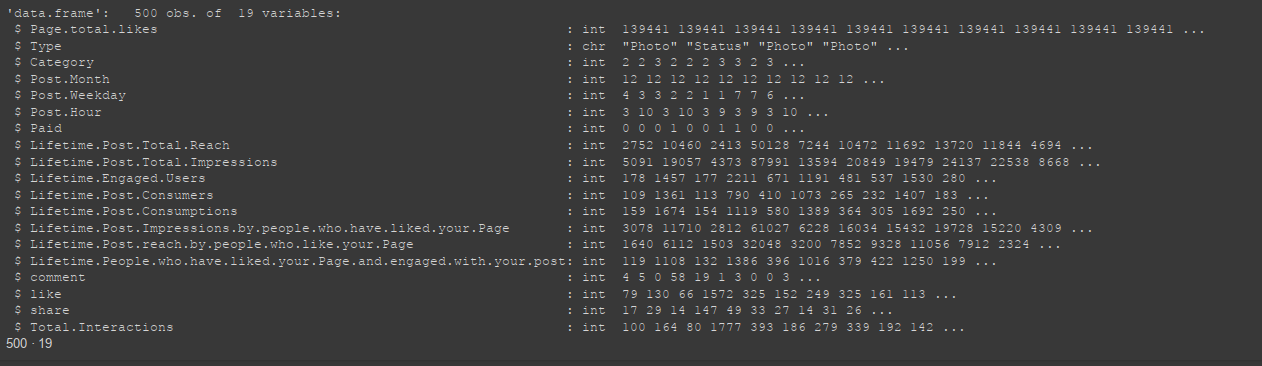
\includegraphics[width=0.8\linewidth]{part23_figures/01.png}
        \caption{Tóm tắt dữ liệu Facebook}
        \label{fig:Tóm tắt dữ liệu Facebook}
    \end{figure}
    \item[\textbf{Bước 2}]: \textbf{Thực hiện kiểm tra về bộ dữ liệu bao gồm: Kiểm tra tính độc lập, Kiểm tra dữ liệu khuyết, và kiểm tra outliners của bộ dữ liệu.}
    
    Hiện tại, bộ dữ liệu chứa rất nhiều biến thông tin, trong phạm vi của đề tài này, chúng tôi sẽ không tiến hành khảo sát tất cả các biến mà chỉ chọn ra 2 biến độc lập để phân tích ANOVA đó là `Category`  và `Paid` có ảnh hưởng đến kết quả số lượt thích của bài viết `like` như thế nào.
    
        \begin{itemize}
            \item Kiểm tra tính độc lập của dữ liệu
                \begin{lstlisting}              
# Kiểm tra tính độc lập của dữ liệu
processed_data = fb_raw[c("Category", "Paid", "like")]
duplicates = fb_raw[duplicated(processed_data), ]
duplicate_counts = table(processed_data[duplicated(processed_data), ])
duplicate_counts
                \end{lstlisting}
                \newpage
                Thực thi đoạn mã trên, ta thấy rằng đối với bộ dữ liệu này, có sự trùng lặp giữa các quan trắc, vậy chúng độc lập với nhau. Vì vậy chúng ta sẽ loại bỏ các điểm này
                \begin{lstlisting}
rm_duplicated_data = processed_data[!duplicated(processed_data),]
processed_data = rm_duplicated_data
dim(processed_data)
                \end{lstlisting}
    Sau bước này, ta thu được 407 samples.

            \item Kiểm tra dữ liệu khuyết
                \begin{lstlisting}
missing_ratio = function(s) {
  round(mean(is.na(s)) * 100, 1)
}
sapply(islander_raw, missing_ratio)
                \end{lstlisting}
                Thực thi đoạn mã trên, ta thấy rằng đối với bộ dữ liệu này, các quan trắc có khuyết đặc trưng, ta tiến hành loại bỏ chúng.
                \begin{lstlisting}
processed_data = na.omit(processed_data)
dim(processed_data)
                \end{lstlisting}
                Thực thi đoạn ma này ta còn lại 405 quan trắc.
            \item Kiểm tra ngoại lai và cực ngoại lai
                Đối với bước này, ta chỉ kiểm tra đối với các biến có giá trị là numerics, như vậy ta sẽ khảo sát các biến \textbf{like}
                \begin{lstlisting}
# Create a box plot
boxplot(processed_data["like"], main="Outliers Analysis", col="lightblue")
                \end{lstlisting}
                \begin{figure}[H]
                    \centering
                    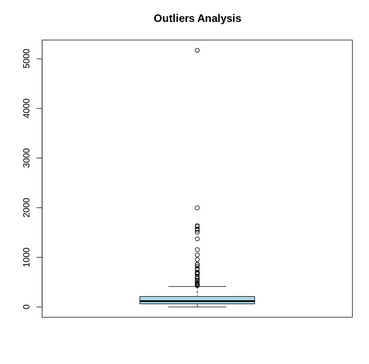
\includegraphics[width=0.8\linewidth]{part23_figures/02.png}
                    \caption{Khảo sát outliners}
                    \label{fig:Khảo sát outliners}
                \end{figure}
                
                Từ biểu đồ hộp, ta có nhận xét sau đây:Nhìn vào biểu đồ này, chúng ta thấy có rất nhiều điểm ngoại lai và cực ngoại lai ở phía trên, chứng tỏ rằng có một số bài đăng trên facebook có sự tương tác rất mạnh.
                
                Tiếp theo là biểu đồ phân phối của biến \textbf{like}
                \begin{figure}[H]
                    \centering
                    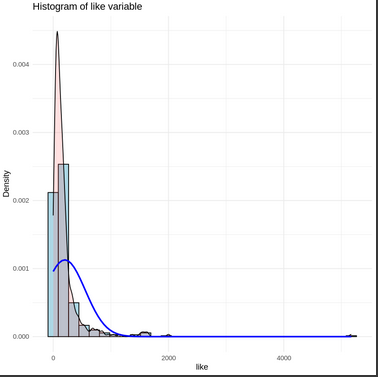
\includegraphics[width=0.8\linewidth]{part23_figures/03.png}
                    \caption{Biểu đồ phân phối biến like}
                    \label{fig:Biểu đồ phân phối biến like}
                \end{figure}
                Nhận xét: Phân bố có vẻ hơi lệch về phía bên trái so với trung bình.
        \end{itemize}
        
    \item [\textbf{Bước 3}]: \textbf{Trực quan hóa dữ liệu và rút ra nhận xét.}
    
        Ta sẽ dùng R để vẽ ra biểu đồ phân bố của dữ liệu
        \begin{lstlisting}
# Đưa về kiểu dữ liệu phù hợp
processed_data$Paid = factor(processed_data$Paid)
processed_data$Category = factor(processed_data$Category)

# Visualize biến Paid
ggplot(processed_data ,aes(x=Paid, y=like, colour=Paid, fill=Paid))+
  geom_jitter(width=0.25)+
  geom_boxplot(alpha=0.25, outlier.alpha=0) +
  stat_summary(fun.y=mean, colour="black", geom="point",
               shape=18, size=3,show.legend = FALSE) +
  theme_classic() +
  theme(legend.position="none")+
  theme(axis.text = element_text(angle=30, hjust=1, vjust=1))
        \end{lstlisting}
            \begin{figure}[H]
                \centering
                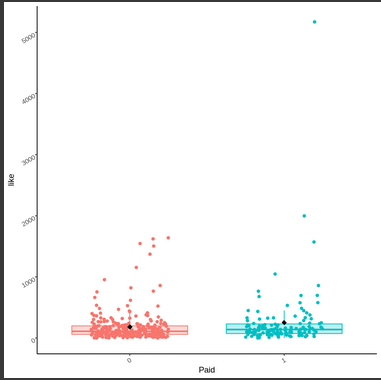
\includegraphics[width=0.8\linewidth]{part23_figures/04.png}
                \caption{Biểu đồ phân bố biến Paid}
                \label{fig:Biểu đồ phân bố biến Paid}
            \end{figure}
        Từ hai đồ thị trên, ta có một số nhận xét như sau:\begin{itemize}
            \item Ở nhóm 0 (Không thuê quảng cáo):Trung vị lớn hơn 0, đa số tập trung trong box; tồn tại ngoại lệ và cực ngoại lệ
            \item Ở nhóm 1 (Có thuê quảng cáo): Trung vị lớn hơn 0 và lớn hơn nhóm không thuê quảng cáo, chứng tỏ rằng việc chi trả tiền cho quảng cáo sẽ mang lại kết quả tích cực hơn.Số lượng ngoại lai và cực ngoại lai ít hơn nhóm 0 nhưng biến động hơn ở phía trên.
            \item Việc chi trả tiền thuê quảng cáo về mặt tổng quan cho hiệu quả tích cực hơn so với không thuê quảng cáo, tuy nhiên không phải lúc nào cũng giúp cho bài post tăng sự tương tác (có nhiều điểm gần điểm 0)

        Tiếp theo ta sẽ biểu diễn cho biến \textbf{Category}:
        \begin{lstlisting}
# Biến Category
ggplot(processed_data ,aes(x=Category, y=like, colour=Category,fill=Category))+
  geom_jitter(width=0.25)+
  geom_boxplot(alpha=0.25, outlier.alpha=0) +
  stat_summary(fun.y=mean, colour="black", geom="point",
               shape=18, size=3,show.legend = FALSE)+
  theme_classic()+
  theme(legend.position="none")+
  theme(axis.text = element_text(angle=30, hjust=1, vjust=1))
        \end{lstlisting}
    \begin{figure}[H]
        \centering
        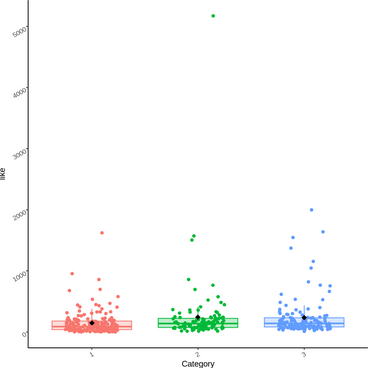
\includegraphics[width=0.8\linewidth]{part23_figures/05.png}
        \caption{Biểu đồ phân bố biến Category}
        \label{fig:Biểu đồ phân bố biến Category}
    \end{figure}
    Nhận xét: Về tổng quan ta thấy rằng các nhóm đa số đều nằm trong khoảng box, vẫn tồn tại các điểm ngoại lai, Tuy nhiên ở chủ đề 2 và 3 cho thấy rằng hiệu quả tích cực hơn nhóm 1 (trung vị cao hơn và biến động ngoại lai rộng hơn)
    Cuối cùng là biến \textbf{Like}
    \begin{figure}[H]
        \centering
        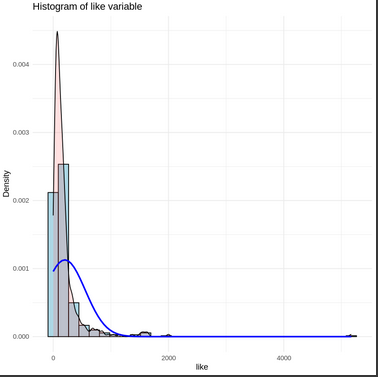
\includegraphics[width=0.8\linewidth]{part23_figures/03.png}
        \caption{Phân phối biến Like}
        \label{fig:Phân phối biến Like}
    \end{figure}
        \begin{enumerate}
            \item \textbf{Thống Kê Mô Tả}:
            \begin{itemize}
                \item \textbf{Giá trị nhỏ nhất}: 0.0
                \item \textbf{Phân vị thứ nhất (Q1)}: 63.0
                \item \textbf{Trung vị (Q2)}: 118.0
                \item \textbf{Giá trị trung bình}: 202.3
                \item \textbf{Phân vị thứ ba (Q3)}: 210.0
                \item \textbf{Giá trị lớn nhất}: 5172.0
            \end{itemize}
        
            \item \textbf{Hình Dạng Phân Bố}:
            \begin{itemize}
                \item Phân bố có độ lệch phải lớn (lệch dương). Điều này thể hiện qua đuôi dài mở rộng về phía các giá trị lớn hơn.
                \item Phần lớn các điểm dữ liệu tập trung ở phía đầu dưới, với đỉnh nhọn gần giá trị nhỏ nhất.
            \end{itemize}
        
            \item \textbf{Xu Hướng Trung Tâm}:
            \begin{itemize}
                \item Trung vị (118.0) thấp hơn đáng kể so với giá trị trung bình (202.3), đây là một dấu hiệu khác của sự lệch.
                \item Các giá trị phân vị thứ nhất và thứ ba cũng cho thấy phần lớn dữ liệu tập trung ở khoảng giá trị thấp.
            \end{itemize}
        
            \item \textbf{Giá Trị Ngoại Lệ}:
            \begin{itemize}
                \item Có một số giá trị ngoại lệ lớn kéo dài đến 5172.0, xa so với phần lớn dữ liệu. Những ngoại lệ này làm ảnh hưởng đến giá trị trung bình, làm cho nó cao hơn so với trung vị.
            \end{itemize}
        
            \item \textbf{Biểu Đồ Mật Độ}:
            \begin{itemize}
                \item Đường màu xanh biểu thị ước lượng mật độ của biến "like".
                \item Biểu đồ mật độ cũng xác nhận sự lệch, với đỉnh cao ở các giá trị thấp và giảm dần về phía các giá trị cao.
            \end{itemize}
\end{enumerate}

\end{itemize}

\subsection{Kiểm định các giả thiết thống kê (ANOVA assumptions)}
Nhắc lại các điều kiện để phân tích ANOVA như sau:
\begin{itemize}
    \item [1.] Các mẫu độc lập
    \item [2.] Biến phụ thuộc là biến liên tục
    \item [3.] Các nhóm có phân phối chuẩn hoặc gần chuẩn, đồng nghĩa với việc kiểm định phương sai các nhóm cho kết quả là đồng nhất.
\end{itemize}

Rõ ràng, theo như phân tích phía trên, bộ dữ liệu chúng ta đã thỏa mãn điều kiện (1) và (2). Để chắc chắn ta sẽ đi kiểm định yêu cầu số (3) bằng cách tiến hành thực hiện các kiểm định sau:
\begin{itemize}
    \item Shapiro-Wilk test
    \item leveneTest
    \item durbinWatsonTest
\end{itemize}

Đầu tiên ta sẽ xây dựng mô hình tương tác bằng dòng lệnh sau
\begin{lstlisting}
# Xây dựng mô hình tương tác
int_model = aov(like~Category * Paid, data = processed_data)
summary(int_model)
\end{lstlisting}

Kết quả thu được:

\begin{lstlisting}
               Df   Sum Sq Mean Sq F value Pr(>F)  
Category        1   584670  584670   4.741 0.0300 *
Paid            1   487829  487829   3.956 0.0474 *
Category:Paid   1      971     971   0.008 0.9293  
Residuals     401 49452484  123323                 
---
Signif. codes:  0 '***' 0.001 '**' 0.01 '*' 0.05 '.' 0.1 ' ' 1
\end{lstlisting}
Với mức ý nghĩa 5\%, ta thấy rằng giữa `Category` và `Paid` có mối quan hệ tương tác với nhau dẫn đến tác động hiệu quả của việc dùng thuốc đối với trí nhớ của người sử dụng. Tiếp tục đi kiểm định các thông số sau:

\begin{lstlisting}
# Shapiro-Wilk test
av_residual = rstandard(int_model)
shapiro.test(av_residual)
# Trực quan bằng QQ plot
qqnorm(av_residual)
qqline(av_residual)
hist(av_residual)
\end{lstlisting}
\begin{figure}[H]
    \centering
    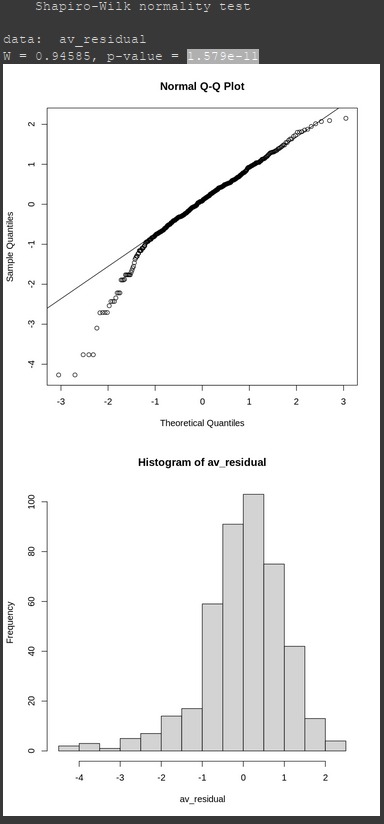
\includegraphics[width=0.5\linewidth]{part23_figures/06.png}
    \caption{Biểu đồ phần dư}
    \label{fig:Biểu đồ phần dư_}
\end{figure}

\newpage
Kết quả như sau:
\begin{lstlisting}
	Shapiro-Wilk normality test

data:  av_residual
W = 0.94585, p-value = 1.579e-11
\end{lstlisting}

Xét giả định
\begin{itemize}
    \item H0: Tuân theo phân phối chuẩn
    \item H1: Không tuân theo phân phối chuẩn
\end{itemize}

Nhận xét: với độ tin cậy 5\% thì với giá trị p-value = 1.579e-11 chúng ta đủ cơ sở bác bỏ H0, vậy sai số có phân phối không chuẩn. Nhìn vào biểu đồ, ta thấy rằng ở phần đuôi kéo dài, nhiều điểm bị kéo lệch ra khỏi đường thẳng,  Khả năng các điểm nhiễu chính là các điểm ngoại lệ (outliners).

Bước tiếp theo ta Kiểm định các nhóm có phương sai đồng nhất hay không
\begin{lstlisting}
leveneTest(int_model)
\end{lstlisting}

Kết quả
\begin{lstlisting}
A anova: 2 x 3 	
Df	F value	Pr(>F)
	<int>	<dbl>	<dbl>
group	5	3.431213	0.004772486
	399	NA	NA
\end{lstlisting}

Giả định:

- H0: Các nhóm có phương sai đồng nhất

- H1: Các nhóm không có phương sai đồng nhất

Nhận xét: Với giá trị p-value = 0.004 < 0.05, ta đủ điều kiện bác bỏ H0, vậy các nhóm có phương sai không đồng nhất.

\newpage
\begin{lstlisting}
# Kiểm định tính độc lập của phần dư
durbinWatsonTest(int_model)
plot(int_model, 1)
\end{lstlisting}

Kết quả 
\begin{figure}[H]
    \centering
    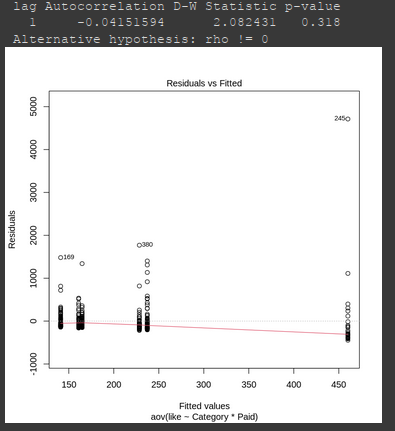
\includegraphics[width=0.8\linewidth]{part23_figures/07.png}
    \caption{Kết quả kiệm định durbinWatsonTest}
    \label{fig:Kết quả kiệm định durbinWatsonTest}
\end{figure}
Với giả định:
\begin{itemize}
    \item H0: Không có sự tương quan (độc lập).
    \item H1: H1: Có sự tương quan (không độc lập).
\end{itemize}

Thì với giá trị p-value = 0.318 (> 0.05) nên không có sự tương quan. Vậy phần dư độc lập

\subsection{Phân tích phương sai k nhân tố}
Với bước kiểm định levene ta thấy rằng mô hình chúng ta không đảm bảo tính chuẩn, tuy nhiên với mức giá trị p=0.047 ta thấy rằng xấp xỉ chuẩn với độ tự tin 0.05. Vì thế, ta vẫn có thể tiếp tục đi phân tích ANOVA.
Tiếp theo chung ta sẽ tiến hành đi phân tích phương sai k nhân tố. Việc này gồm các bước sau:
\begin{itemize}
    \item [1.] Kiểm tra sự tương tác
    \item [2.] Phân tích ảnh hưởng đơn
    \begin{itemize}
        \item Phân tích ảnh hưởng đơn của quảng cáo ở mỗi loại thể loại
        \item Phân tích ảnh hưởng đơn của thể loại trong việc sử dụng quảng cáo
    \end{itemize}
    \item [3.] Phân tích ảnh hưởng chính
    \begin{itemize}
        \item Phân tích ảnh hưởng chính của Quảng cáo với hiệu quả của bài post
        \item Phân tích ảnh hưởng chính của Thể loại với hiệu quả của bài post
    \end{itemize}
\end{itemize}

Sau đây là các bước chi tiết:
\begin{itemize}
    \item \textbf{Bước 1: Xây dựng mô hình tương tác (interaction model) và kiểm tra tương tác của các biến}

    \begin{lstlisting}
int_model = aov(like~Category * Paid, data = processed_data)
summary(int_model)
plot(interactionMeans(int_model))
    \end{lstlisting}

    Kết quả
    \begin{figure}[H]
        \centering
        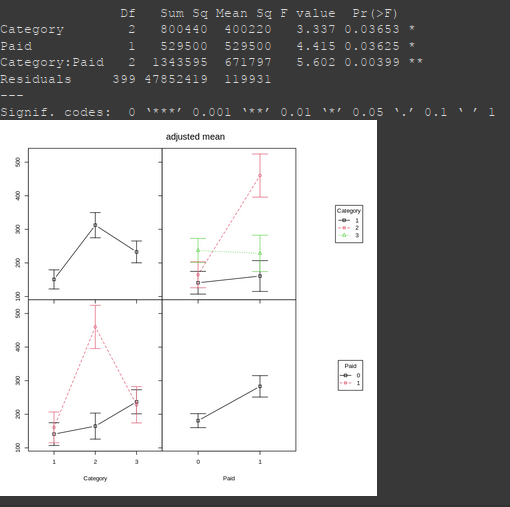
\includegraphics[width=0.8\linewidth]{part23_figures/08.png}
        \caption{Tương tác giữa các biến trong mô hình}
        \label{fig:Tương tác giữa các biến trong mô hình}
    \end{figure}
Ta rút ra một số nhận xét dựa trên kết quả như sau: 

- Với mức ý nghĩa 5\%,  Kết quả ANOVA cho thấy các yếu tố "Category" và "Paid" đều có ảnh hưởng đáng kể đến biến phụ thuộc (p-value < 0.05).Tương tác giữa "Category" và "Paid" cũng có ảnh hưởng đáng kể (p-value < 0.01).

- Đối với biểu đồ bên trái:
    \begin{itemize}
        \item [+]  Đồ thị trên cùng bên trái (Thể hiện mối quan hệ giữa "Category" và giá trị trung bình điều chỉnh): "Category 2" có giá trị trung bình cao nhất, trong khi "Category 1" và "Category 3" có giá trị trung bình thấp hơn.
        \item [+]  Đồ thị dưới cùng bên trái (Thể hiện mối quan hệ giữa "Category" và "Paid"):
        \begin{itemize}
            \item "Category 2" có giá trị trung bình cao nhất khi "Paid" = 0, và giảm khi "Paid" = 1.
            \item Khi Paid = 0, ta thấy rằng có sự tăng trưởng khi Category đi từ 1 đến 3. Ngược lại "Paid" = 1 thì kết quả lúc tăng lúc giảm
            \item Về tổng quan thì Paid = 1 sẽ cho kết quả tốt hơn, đặc biệt là category 2.
        \end{itemize}
    \end{itemize}

- Đối với biểu đồ bên phải:
    \begin{itemize}
        \item [+] Đồ thị trên cùng bên phải (Thể hiện mối quan hệ giữa "Paid" và giá trị trung bình điều chỉnh cho các nhóm "Category"): Nhóm category2 cho thấy hiệu quả vượt bậc khi Paid = 1, trong khi 2 nhóm còn lại thì không có sự thay đổi không đáng kể (tăng giảm rất ít).
        \item [+] Đồ thị dưới cùng bên phải (Thể hiện mối quan hệ giữa "Paid" và giá trị trung bình điều chỉnh.): Tương tác giữa "Category" và "Paid" cho thấy sự thay đổi trong giá trị trung bình giữa các nhóm "Category" phụ thuộc vào trạng thái "Paid".
    \end{itemize}
Ta có kết luận sau đây:
    \begin{itemize}
        \item Cả "Category" và "Paid" đều ảnh hưởng đáng kể đến giá trị trung bình điều chỉnh của biến phụ thuộc.
        \item Tương tác giữa "Category" và "Paid" cho thấy sự thay đổi trong giá trị trung bình giữa các nhóm "Category" phụ thuộc vào trạng thái "Paid".
    \end{itemize}

\item \textbf{Bước 2: Phân tích ảnh hưởng đơn}

        Để phân tích ảnh hưởng đơn ta sẽ sử dụng hàm \textbf{testInteractions} để tiến hành phân tích. Sau đây là các bước chi tiết
    \begin{itemize}
        \item Phân tích ảnh hưởng đơn của quảng cáo ở mỗi loại thể loại
            \begin{lstlisting}
testInteractions(int_model, fixed = "Paid", across = "Category")
            \end{lstlisting}
            Kết quả:
            \begin{figure}[H]
                \centering
                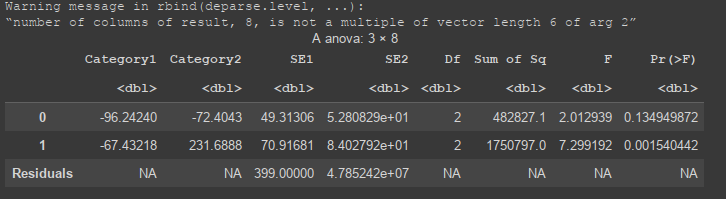
\includegraphics[width=0.8\linewidth]{part23_figures/09.png}
                \caption{Kết quả tương tác giữa Paid và Category}
                \label{fig:Kết quả tương tác giữa Paid và Category}
            \end{figure}
            Với các giả định như sau:
            \begin{itemize}
                \item H0:  Thuê quảng cáo Không ảnh hưởng đến hiệu quả tương tác bài post
                \item H1:  Thuê quảng cáo Có ảnh hưởng đến hiệu quả của tương tác bài post
            \end{itemize}
            Ta rút ra kết luận như sau: Với kết quả phân tích ta có một số nhận xét như sau, với độ tin cậy 5\% thì: Thuê quảng cáo có ảnh hưởng đến kết quả của loại tương tác bài post ở các thể loại
        \item Phân tích ảnh hưởng đơn của thể loại ở việc thuê quảng cáo
            \begin{lstlisting}
testInteractions(int_model, fixed = "Category", across = "Paid")
            \end{lstlisting}
            \begin{figure}[H]
                \centering
                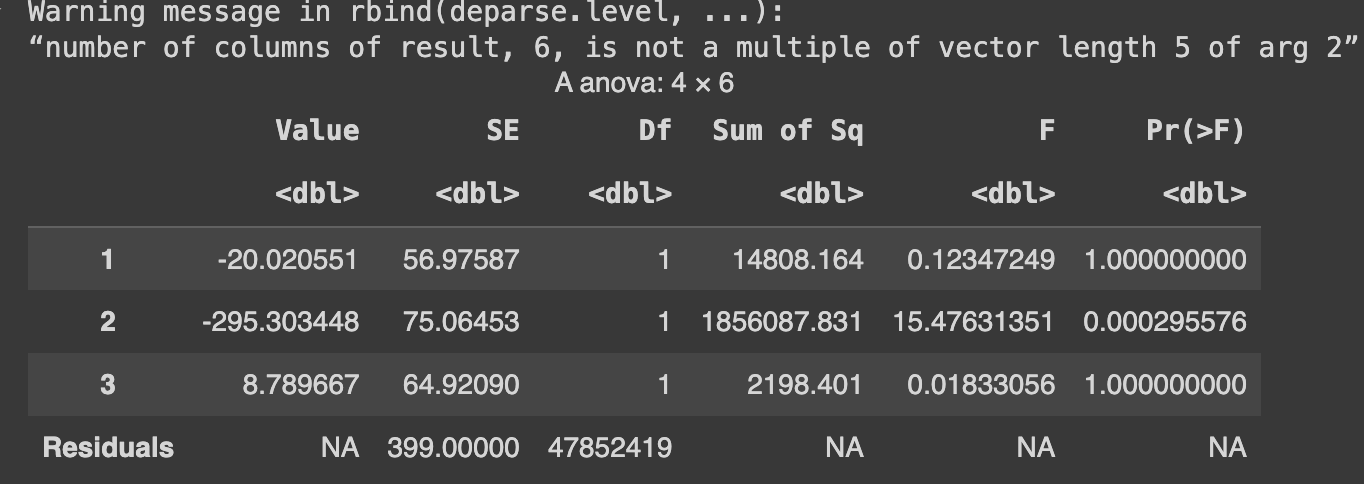
\includegraphics[width=0.8\linewidth]{part23_figures/10.png}
                \caption{Ảnh hưởng đon giữa thể loại ở việc thuê quảng cáo}
                \label{fig:Ảnh hưởng đon giữa thể loại ở việc thuê quảng cáo}
            \end{figure}
            Tương tự như ở phía trên, ta có các giả định như sau:
            \begin{itemize}
                \item H0: Thể loại không có sự tương tác trong việc thuê quảng cáo
                \item H1: Thể loại có sự tương tác trong việc thuê quảng cáo
            \end{itemize}
        Ta rút ra kết luận như sau: Với kết quả phân tích ta có một số nhận xét như sau, với độ tin cậy 5\% thì: Chỉ có thể loại thứ 2 thể hiện rõ sự tương tác với \textbf{Paid}, các trường hợp còn lại là không thể hiện sự tương tác.

        \item Phân tích ảnh hưởng đơn giữa các nhóm thể loại ứng với việc thuê quảng cáo hay không thuê quảng cáo
        
        Việc phân tích sự tương tác của các nhóm trong cùng một điều kiện nhất định cũng có ý nghĩa rất quan trọng trong thống kê, từ đó sẽ hiểu rõ hơn về từng tác dụng của từng loại và từng nhóm
        \begin{lstlisting}
options(contrasts = c(unordered="contr.sum", ordered="contr.poly"))
one_vs_two = list(Category = c(1, -1, 0))
one_vs_three = list(Category = c(1, 0, -1))
two_vs_three = list(Category = c(0, 1, -1))
        \end{lstlisting}

        Đầu tiên, ta sẽ đi phân tích ảnh hưởng của nhóm Category1 và Category2
        \begin{lstlisting}
testInteractions(int_model, custom = c(one_vs_two), fixed = "Paid", adjustment = "bonferroni")
        \end{lstlisting}
        Kết quả:
        \begin{figure}[H]
            \centering
            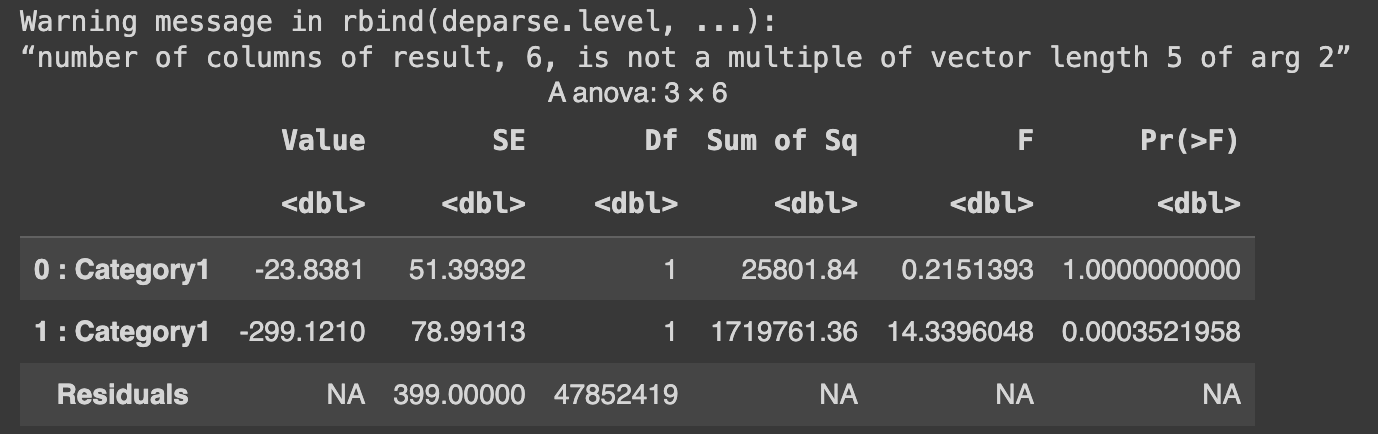
\includegraphics[width=0.8\linewidth]{part23_figures/11.png}
            \caption{Tương tác giữa nhóm 1 và 2 ở mỗi liều lượng}
            \label{Tương tác giữa nhóm 1 và 2 ở mỗi liều lượng}
        \end{figure}
        Ta có giả định như sau:
        \begin{itemize}
            \item H0: Không có sự khác nhau giữa nhóm 1 và nhóm 2
            \item H1: Có sự khác nhau giữa nhóm 1 và nhóm 2
        \end{itemize}
        Ta rút ra kết luận như sau: Với kết quả phân tích ta có một số nhận xét như sau, với độ tin cậy 5\% thì: Có sự tương tác có ý nghĩa thống kê ở việc thuê quảng cáo giữa nhóm 1 và nhóm 2.

        
        Tiếp theo là nhóm Category1 và Category3
        
        \begin{lstlisting}
testInteractions(int_model, custom = c(one_vs_three), fixed = "Paid", adjustment = "bonferroni")
        \end{lstlisting}
        Kết quả:
        \begin{figure}[H]
            \centering
            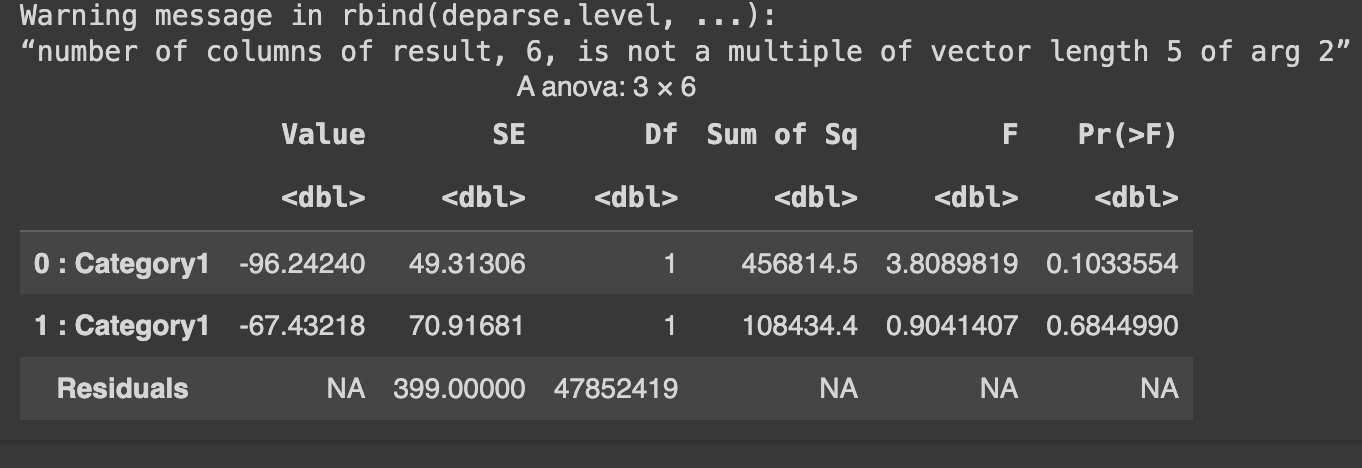
\includegraphics[width=0.5\linewidth]{part23_figures/12.png}
            \caption{Tương tác giữa nhóm 1 và 3}
            \label{fig:Tương tác giữa nhóm 1 và 3}
        \end{figure}
        Với các giả định tương tự với nhóm 1 và 2, ta có kết luận như sau:
        \begin{itemize}
            \item Có sự tương tác có ý nghĩa thống kê ở việc thuê quảng cáo giữa nhóm 1 và nhóm 3
            \item Có sự tương tác có ý nghĩa thống kê ở việc không thuê quảng cáo giữa nhóm 1 và nhóm 3
        \end{itemize}
        Cuối cùng là giữa nhóm 2 và 3
        \begin{lstlisting}
testInteractions(int_model, custom = c(two_vs_three), fixed = "Paid", adjustment = "bonferroni")
        \end{lstlisting}
        Kết quả:
        \begin{figure}[H]
            \centering
            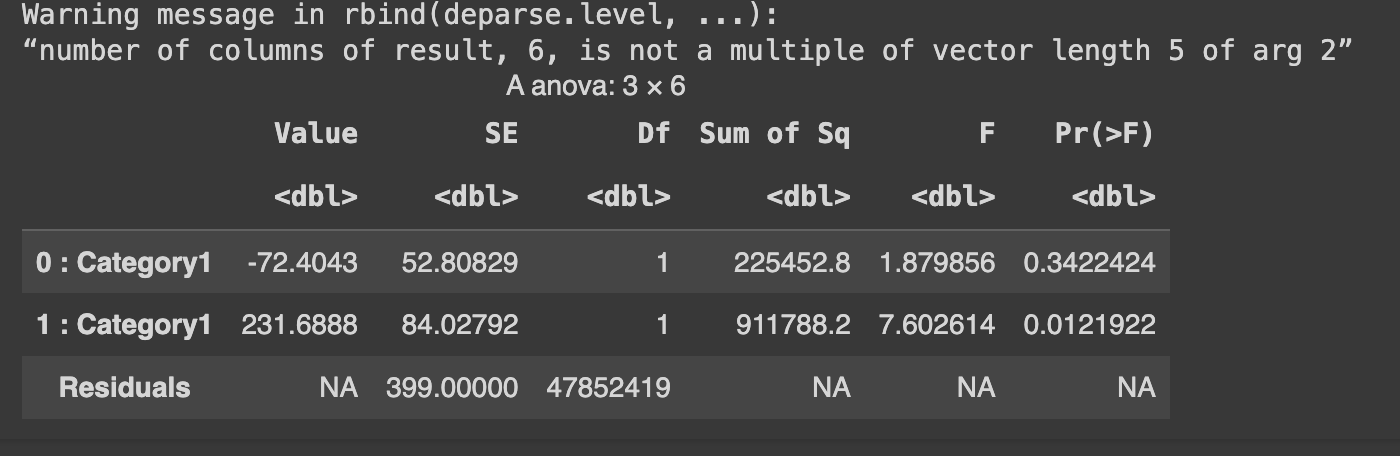
\includegraphics[width=0.5\linewidth]{part23_figures/13.png}
            \caption{Tương tác giữa nhóm 2 và 3}
            \label{fig:Tương tác giữa nhóm 2 và 3}
        \end{figure}
         Với các giả định tương tự với nhóm 1 và 2, ta có kết luận như sau: Với độ tin cậy 5\% thì \begin{itemize}
             \item Có sự tương tác có ý nghĩa thống kê ở việc thuê quảng cáo giữa nhóm 2 và nhóm 3
             \item Có sự tương tác có ý nghĩa thống kê ở việc không thuê quảng cáo giữa nhóm 2 và nhóm 3
         \end{itemize}
    \end{itemize}
    Từ việc phân tích trên, ta có kết luận như sau: Việc thuê quảng cáo chỉ cho kết quả tốt hơn ở nhóm 1 và 2. Các nhóm còn lại việc chi tiền cho quảng cáo và không chi tiền đều cho kết quả như nhau, Khả năng cao mức ảnh hưởng này sẽ giải thích bới một yếu tố khác mà ta chưa khảo sát (như content chẳng hạn).

    \item Phân tích ảnh hưởng đơn giữa quảng cáo ứng với các nhóm thể loại
    \begin{lstlisting}
options(contrasts = c(unordered="contr.sum", ordered="contr.poly"))
no_vs_yes = list(Paid = c(1, -1))
testInteractions(int_model, custom = c(no_vs_yes), fixed = "Category", adjustment = "bonferroni")
    \end{lstlisting}
   Kết quả:
   \begin{figure}[H]
       \centering
       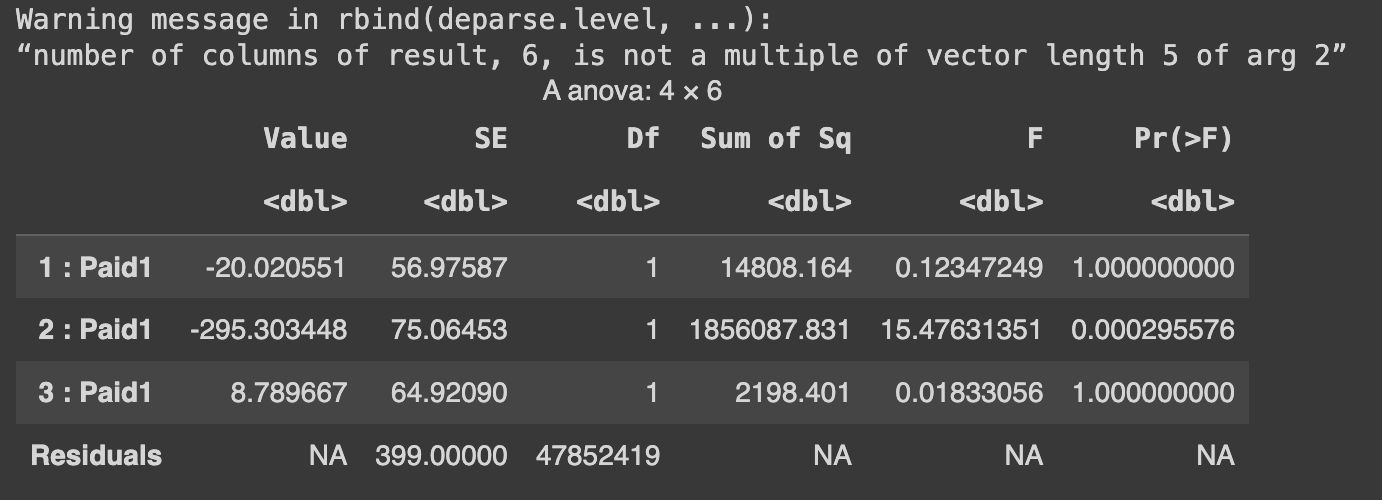
\includegraphics[width=0.8\linewidth]{part23_figures/14.png}
       \caption{Ảnh hưởng đơn giữa quảng cáo ứng với các nhóm thể loại}
       \label{fig:Ảnh hưởng đơn giữa quảng cáo ứng với các nhóm thể loại}
   \end{figure}
    Với giả định sau:
        \begin{itemize}
            \item H0: Không có sự khác nhau trong tương tác hiệu quả giữa việc thuê quảng cáo và không thuê quảng cáo
            \item H1: Có sự khác nhau trong tương tác hiệu quả giữa việc thuê quảng cáo và không thuê quảng cáo
        \end{itemize}
    Với độ tin cậy 5\% thì: Ở thể loại 1 và 3, chỉ ra không có sự khác nhau hiệu quả giữa việc thuê và không thuê quảng cáo, trong khi đó thể loại 2 cho thấy sự khác nhau này về mặt thống kê.

    \item \textbf{Bước 3: Phân tích ảnh hưởng chính}

    Ở bước này ta sẽ thực hiện 2 phân tích:
    \begin{itemize}
        \item Phân tích ảnh hưởng chính của Paid với hiệu quả của bài post thông qua số lượt like
        \item Phân tích ảnh hưởng chính của Category với hiệu quả của bài post thông qua lượt like
    \end{itemize}
    Với mỗi bước, ta sẽ thực hiện các công việc sau:
    \begin{itemize}
        \item Xây dựng mô hình
        \item Kiểm định các giả thiết của mô hình
        \item Kiểm định trung bình của các nhóm
        \item Nhận xét
    \end{itemize}
    Sau đây là các bước phân tích cụ thể:
    \begin{itemize}
        \item \textbf{Bước 3.1: Phân tích ảnh hưởng chính của Paid với hiệu quả của bài post thông qua số lượt like}
        \begin{lstlisting}
paid_model = aov(like~Paid, data = processed_data)
summary(paid_model)
        \end{lstlisting}
        Kết quả:
        \begin{lstlisting}
            Df   Sum Sq Mean Sq F value Pr(>F)  
Paid          1   439911  439911    3.54 0.0606 .
Residuals   403 50086044  124283                 
---
Signif. codes:  0 '***' 0.001 '**' 0.01 '*' 0.05 '.' 0.1 ' ' 1
        \end{lstlisting}
        Nhận xét: Với mức ý nghĩa 0.05, ta thấy rằng Paid không có ý nghĩa trong việc giải thích mô hình, tuy nhiên chúng ta vẫn đi kiểm định các giả thiết phía sau (vì với mức ý nghĩa 0.06 cũng khá là gần với 0.05)

        Tiếp theo tiến hành kiểm định các giả thuyết
        \begin{lstlisting}
# Shapiro-Wilk test
av_residual = rstandard(paid_model)
shapiro.test(av_residual)

# Trực quan bằng QQ plot
qqnorm(av_residual)
qqline(av_residual)
hist(av_residual)
        \end{lstlisting}
        Kết quả:
\begin{figure}
    \centering
    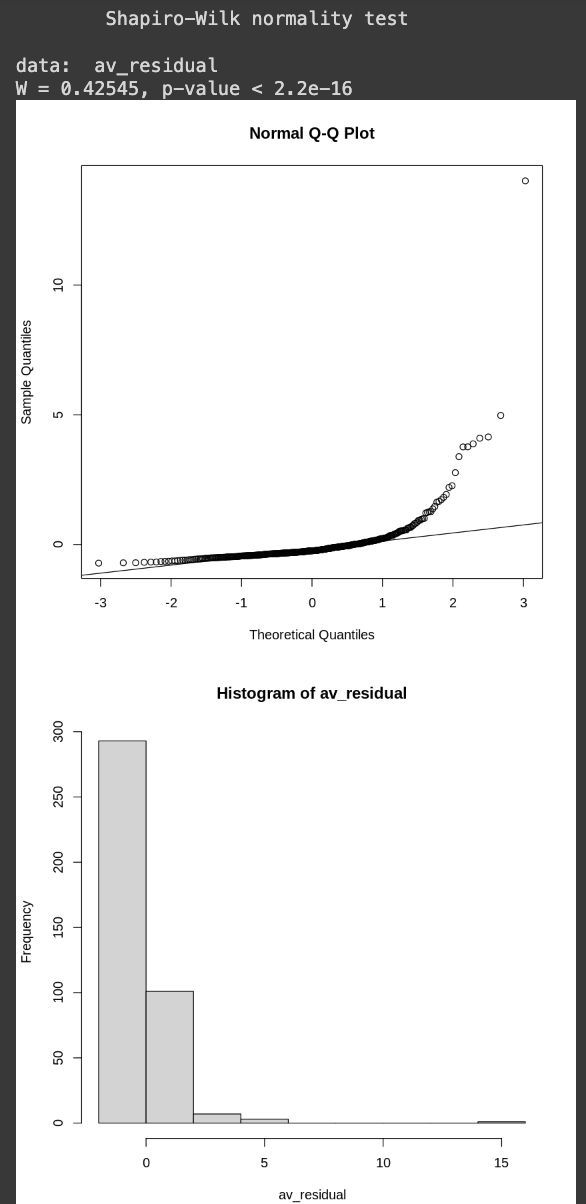
\includegraphics[width=0.6\linewidth]{part23_figures/15.png}
    \caption{Kết quả kiểm định Shapiro-Wilk test}
    \label{fig:Kết quả kiểm định Shapiro-Wilk test}
\end{figure}
        Với giả định:
        \begin{itemize}
            \item H0: Phần dư Tuân theo phân phối chuẩn.
            \item H1: Phần dư Không tuân theo phân phối chuẩn.
        \end{itemize}
        Nhận xét: với độ tin cậy 5\% thì với giá trị p-value = 2.2e-16 chúng ta đủ cơ sở bác bỏ H0, vậy sai số có phân phối không chuẩn. Nhìn vào biểu đồ, ta thấy rằng ở phần đuôi kéo dài, có nhiều điểm bị kéo lệch ra khỏi đường thẳng đặc biệt là đuôi phía trên --> Khả năng các điểm nhiễu chính là các điểm ngoại lệ (outliners), biểu đồ lệch chuẩn

    \begin{lstlisting}
# Kiểm định các nhóm có phương sai đồng nhất hay không
leveneTest(paid_model)
    \end{lstlisting}
    Kết quả:
    \begin{lstlisting}
        A anova: 2 x 3
Df	F value	Pr(>F)
<int>	<dbl>	<dbl>
group	1	2.460602	0.1175189
        403	NA	NA

    \end{lstlisting}
    Với giả định:
    \begin{itemize}
        \item Các nhóm có phương sai đồng nhất.
        \item Các nhóm không có phương sai đồng nhất.
    \end{itemize}
    Nhận xét: Với giá trị p-value = 0.1175189 > 0.05, ta không đủ điều kiện bác bỏ H0, vậy các nhóm có phương sai đồng đồng nhất.
    \end{itemize}
    \begin{lstlisting}
# Kiểm định tính độc lập của phần dư
durbinWatsonTest(paid_model)
plot(paid_model, 1)
    \end{lstlisting}
    Kết quả:
    \begin{figure}[H]
        \centering
        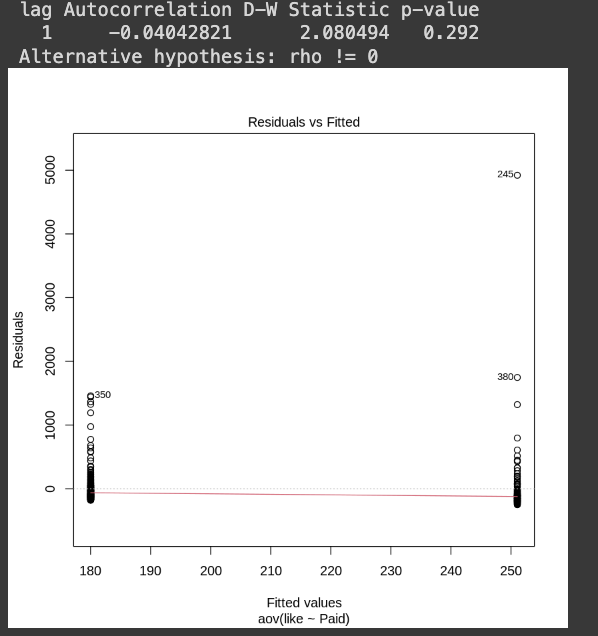
\includegraphics[width=0.8\linewidth]{part23_figures/16.png}
        \caption{Kiểm định durbinWatsonTest}
        \label{fig:Kiểm định durbinWatsonTest}
    \end{figure}
    Với giả định:
    \begin{itemize}
        \item H0: Không có sự tương quan (độc lập)
        \item H1: Có sự tương quan (không độc lập)
    \end{itemize}
    Nhận xét: Với giá trị p-value = 0.292 nên không có sự tương quan.

Măc dù với điều kiện phương sai giữa các nhóm không đồng nhất nên sẽ không tiến hành phân tích ANOVA được, tuy nhiên về mặc trực quan hóa dữ liệu, ta thấy rằng đồ thị phân bố dạng gần chuẩn, nên ta sẽ tiếp tục đi phân tích các yếu tố ANOVA.
\newpage

    \begin{lstlisting}
with(processed_data, pairwise.t.test(like, Paid, p.adj = "bonferroni"))
TukeyHSD(aov(like~Paid, data=processed_data), conf.level = 0.95)
plot(TukeyHSD(aov(like~Paid, data=processed_data), conf.level = 0.95))
    \end{lstlisting}
    Kết quả:
    \begin{figure}[H]
        \centering
        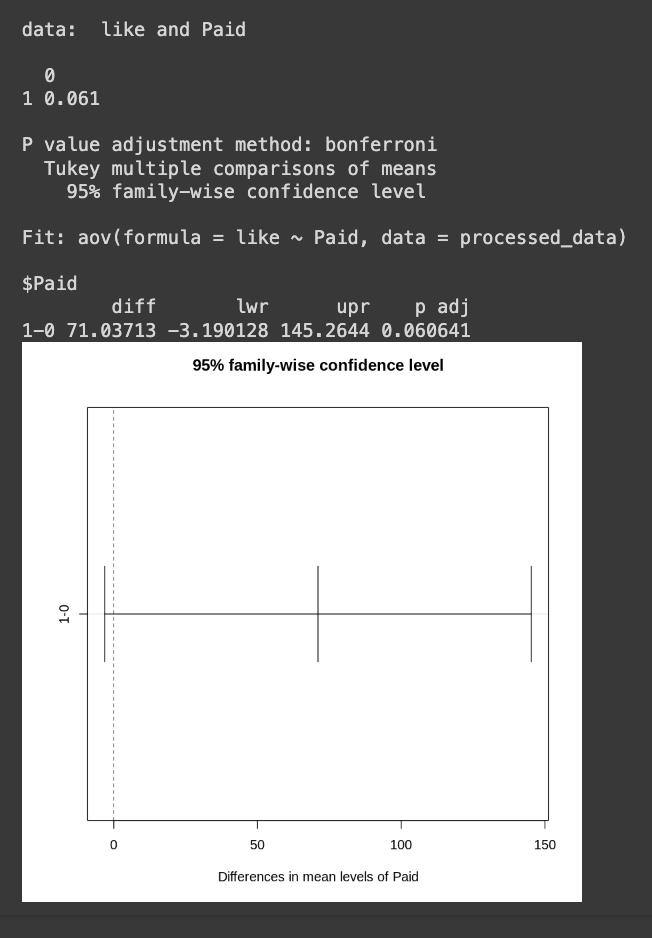
\includegraphics[width=0.8\linewidth]{part23_figures/17.png}
        \caption{Kiểm định Tukey's}
        \label{fig:Kiểm định Tukey's}
    \end{figure}
    Với giả định:
    \begin{itemize}
        \item H0: Các giá trị trung bình giữa các cặp bằng nhau
        \item H1: Các giá trị trung bình giữa các cặp không bằng nhau
    \end{itemize}
    Nhìn vào kết quả ta có: \begin{itemize}
        \item Nhìn vào kết quả ta có: p-value=0.060641 có giá trị lớn hơn 0.05 (độ tin cậy 95\%) nên ta không có cơ sở để bác bỏ H0. Vậy rõ ràng giữa các nhóm này có giá trị trung bình là như nhau. Nghĩa là các nhóm có quảng cáo hay không quảng cáo thì độ hiệu quả là như nhau thông qua số lượng lượt like.
        \item Nhìn vào kết quả và hình vẽ ta cũng thấy ngay giữa nhóm có mức độ hiệu quả trung bình như nhau (đồ thị cắt điểm 0)
    \end{itemize}
Vì chỉ có 2 nhóm nên ta sẽ không tiến hành phân tích tương tác nhóm. Như vậy, ta có kết luận như sau: Việc chi tiền cho quảng cáo hay không cũng chỉ cho cùng một kết quả như nhau (do trung bình như nhau).

\item \textbf{Bước 3.2: Phân tích ảnh hưởng chính của Category với hiệu quả của bài post thông qua lượt like}
    \begin{lstlisting}
category_model = aov(like~Category, data = processed_data)
summary(category_model)
    \end{lstlisting}

Kết quả:
    \begin{lstlisting}
                         Df   Sum Sq Mean Sq F value Pr(>F)  
Category      2   800440  400220   3.236 0.0404 *
Residuals   402 49725514  123695                 
---
Signif. codes:  0 '***' 0.001 '**' 0.01 '*' 0.05 '.' 0.1 ' ' 1
    \end{lstlisting}
Nhận xét: Với mức ý nghĩa 0.05, ta thấy rằng Category có ý nghĩa trong việc giải thích mô hình

\begin{lstlisting}
# Shapiro-Wilk test
av_residual = rstandard(category_model)
shapiro.test(av_residual)

# Trực quan bằng QQ plot
qqnorm(av_residual)
qqline(av_residual)
hist(av_residual)
\end{lstlisting}
Kết quả:
\begin{figure}[H]
    \centering
    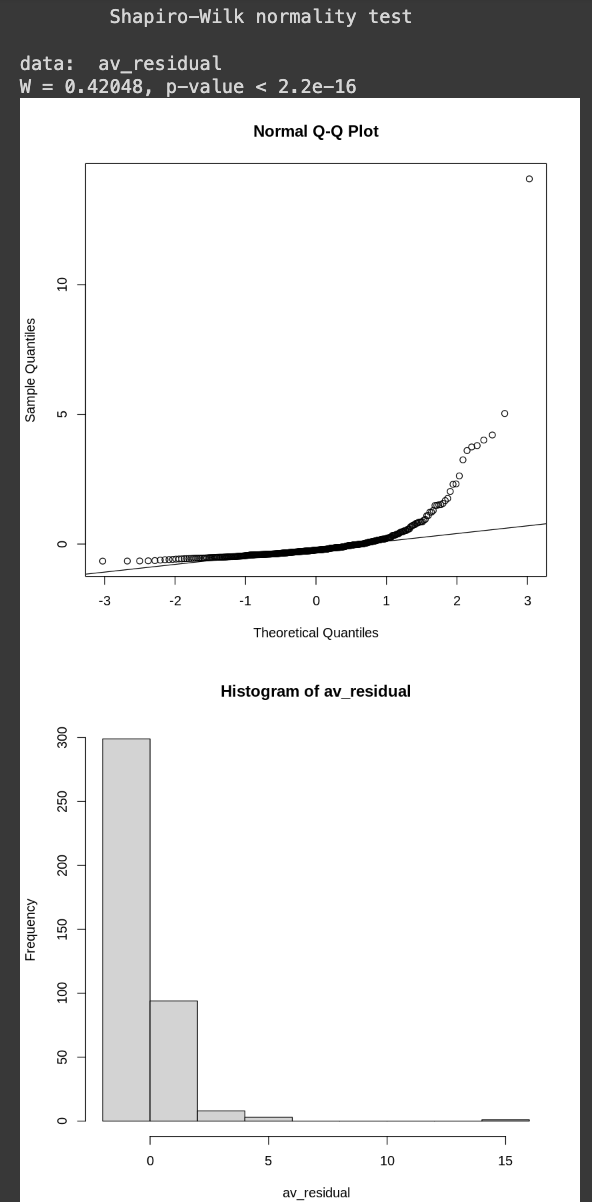
\includegraphics[width=0.6\linewidth]{part23_figures/18.png}
    \caption{Kết quả Shapiro-Wilk test và đồ thị phân phối }
    \label{fig:Kết quả Shapiro-Wilk test và đồ thị phân phối }
\end{figure}
Với các giả định:
    \begin{itemize}
        \item H0: Phần dư tuân theo phân phối chuẩn.
        \item H1: Phần dư không tuân theo phân phối chuẩn
    \end{itemize}
Nhận xét: với độ tin cậy 5\% thì với giá trị p-value = 2.2e-16 chúng ta đủ cơ sở bác bỏ H0, vậy sai số có phân phối không chuẩn. Nhìn vào biểu đồ, ta thấy rằng ở phần đuôi kéo dài, có nhiều điểm bị kéo lệch ra khỏi đường thẳng đặc biệt là đuôi phía trên, Khả năng các điểm nhiễu chính là các điểm ngoại lệ (outliners), biểu đồ lệch chuẩn

    \begin{lstlisting}
# Kiểm định các nhóm có phương sai đồng nhất hay không
leveneTest(category_model)
    \end{lstlisting}
Kết quả:
\begin{lstlisting}
A anova: 2 x 3
Df	F value	Pr(>F)
<int>	<dbl>	<dbl>
group	2	1.191298	0.3048969
        402	NA	NA

\end{lstlisting}
Với các giả định:
    \begin{itemize}
        \item H0: Các nhóm có phương sai đồng nhất
        \item H1: Các nhóm không có phương sai đồng nhất
    \end{itemize}
Nhận xét: Với giá trị p-value = 0.3048969 > 0.05, ta không đủ điều kiện bác bỏ H0, vậy các nhóm có phương sai đồng nhất.

\begin{lstlisting}
# Kiểm định tính độc lập của phần dư
durbinWatsonTest(category_model)
plot(category_model, 1)
\end{lstlisting}

Kết quả:
\begin{figure}
    \centering
    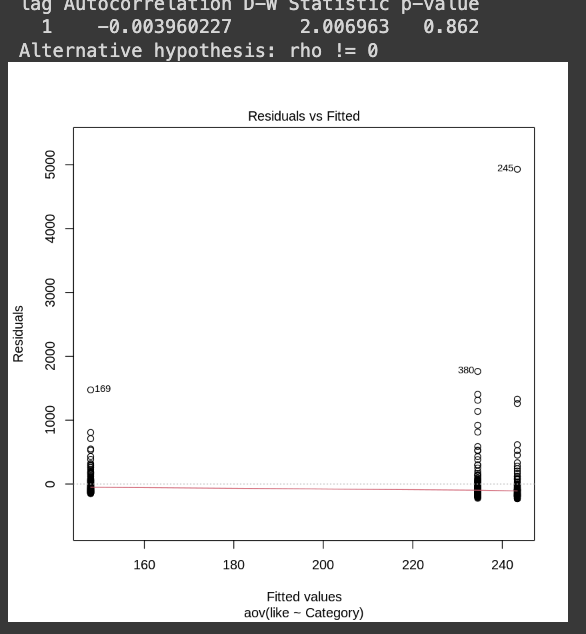
\includegraphics[width=0.8\linewidth]{part23_figures/19.png}
    \caption{Kiểm định durbinWatsonTest}
    \label{fig:Kiểm định durbinWatsonTest_}
\end{figure}
Với các giả định:
    \begin{itemize}
        \item H0: Không có sự tương quan (độc lập)
        \item H1: Có sự tương quan (không độc lập)
    \end{itemize}
Nhận xét: Nhận xét: Với giá trị p-value = 0.87 nên không có sự tương quan.
Măc dù với điều kiện phương sai giữa các nhóm không đồng nhất nên sẽ không tiến hành phân tích ANOVA được, tuy nhiên về mặc trực quan hóa dữ liệu, ta thấy rằng đồ thị phân bố dạng gần chuẩn, nên ta sẽ tiếp tục đi phân tích các yếu tố ANOVA.

\begin{lstlisting}
# Kiểm định độ hiệu quả trung bình giữa các nhóm category
with(processed_data, pairwise.t.test(like, Category, p.adj = "bonferroni"))
TukeyHSD(aov(like~Category, data=processed_data), conf.level = 0.95)
plot(TukeyHSD(aov(like~Category, data=processed_data), conf.level = 0.95))
\end{lstlisting}
Kết quả:
\begin{figure}[H]
    \centering
    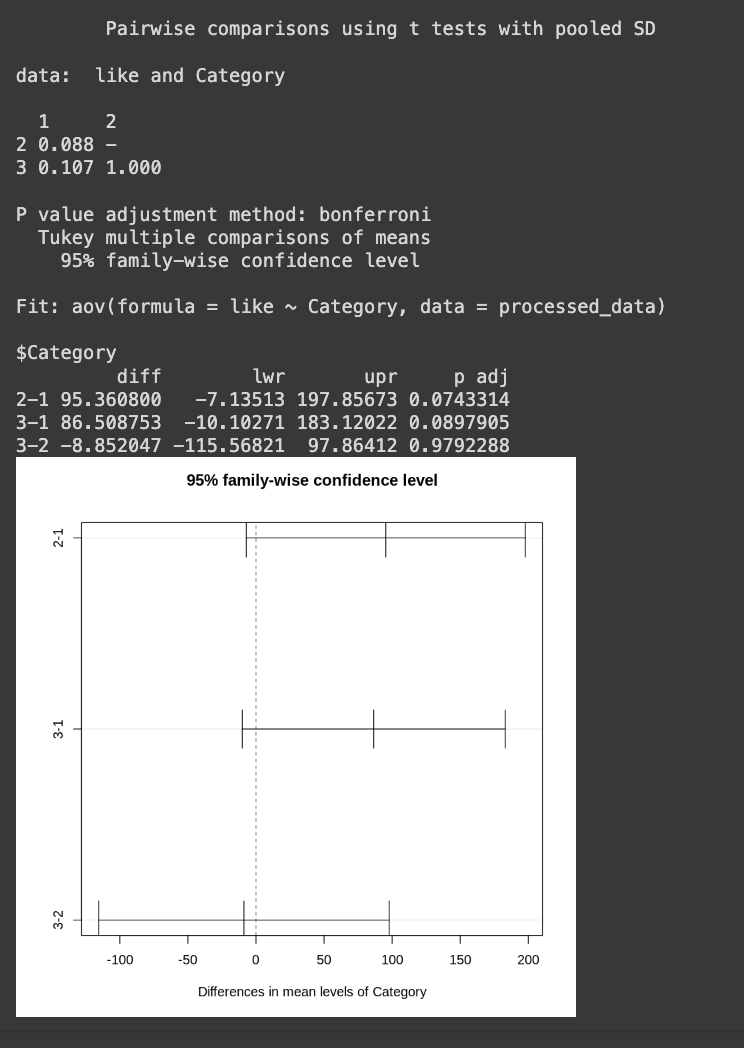
\includegraphics[width=0.5\linewidth]{part23_figures/20.png}
    \caption{Kết quả kiểm định giá trị trung bình}
    \label{fig:Kết quả kiểm định giá trị trung bình}
\end{figure}

Với các giả thuyết:
    \begin{itemize}
        \item H0: Các giá trị trung bình giữa các cặp bằng nhau
        \item H1: Các giá trị trung bình giữa các cặp không bằng nhau
    \end{itemize}
    Nhìn vào kết quả ta có:
    \begin{itemize}
        \item Nhìn vào kết quả ta có: Tất cả các nhóm đều có p-value > 0.05 nên các mức độ trung bình giữa các cặp là như nhau.
        \item Nhìn vào kết quả và hình vẽ ta cũng thấy ngay giữa các cặp có mức độ hiệu quả trung bình như nhau (đồ thị cắt điểm 0)
    \end{itemize}
\end{itemize}
\subsection{Xây dựng và kiểm định mô hình cộng (Additive model)}
\begin{lstlisting}
# Xây dựng mô hình cộng
add_model = aov(like~Category + Paid, processed_data)
summary(add_model)
\end{lstlisting}

Kết quả
\begin{lstlisting}
                 Df   Sum Sq Mean Sq F value  Pr(>F)   
Category      1   838265  838265   8.206 0.00435 **
Paid          1   673770  673770   6.596 0.01051 * 
Residuals   495 50564590  102151                   
---
Signif. codes:  0 '***' 0.001 '**' 0.01 '*' 0.05 '.' 0.1 ' ' 1
\end{lstlisting}

Nhận xét: Với p-value=5\%, các biến đều có ý nghĩa trong giải thích mô hình. Ta tiến hành kiểm định Shapiro và Breusch-Pagan

\begin{lstlisting}
# Shapiro-Wilk test
av_residual = rstandard(add_model)
shapiro.test(av_residual)

# Trực quan bằng QQ plot
qqnorm(av_residual)
qqline(av_residual)
hist(av_residual)
\end{lstlisting}

Kết quả:
\begin{lstlisting}
	Shapiro-Wilk normality test

data:  av_residual
W = 0.43469, p-value < 2.2e-16
\end{lstlisting}

\begin{figure}[H]
    \centering
    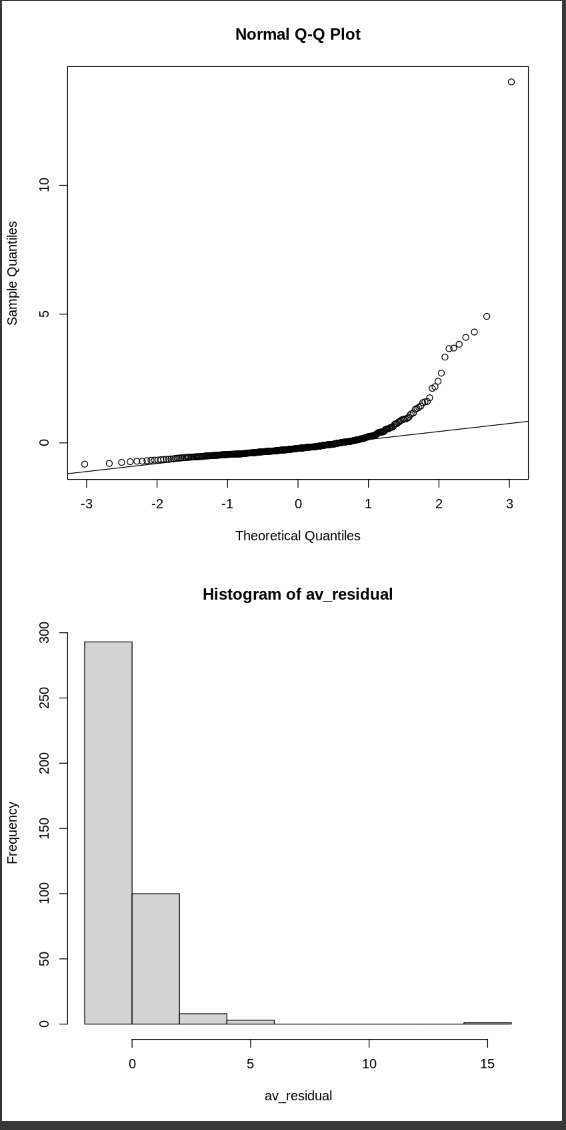
\includegraphics[width=0.6\linewidth]{part23_figures/21.png}
    \caption{Shapiro test và biểu đồ chuẩn của phần dư}
    \label{fig:Shapiro test và biểu đồ chuẩn của phần dư}
\end{figure}

Với các giả định:
    \begin{itemize}
        \item Phần dư H0: Tuân theo phân phối chuẩn
        \item H1: Phần dư Không tuân theo phân phối chuẩn
    \end{itemize}
Nhận xét: với độ tin cậy 5\% thì với giá trị p-value = 2.2e-16 chúng ta đủ cơ sở bác bỏ H0, vậy sai số có phân phối không chuẩn. Nhìn vào biểu đồ, ta thấy rằng ở phần đuôi kéo dài, có nhiều điểm bị kéo lệch ra khỏi đường thẳng đặc biệt là đuôi phía trên --> Khả năng các điểm nhiễu chính là các điểm ngoại lệ (outliners), biểu đồ lệch chuẩn

\begin{lstlisting}
# Kiểm định tính độc lập của phần dư
durbinWatsonTest(add_model)
plot(add_model, 1)
\end{lstlisting}

Kết quả:
\begin{lstlisting}
lag Autocorrelation D-W Statistic p-value
   1     -0.03610975       2.07151   0.428
 Alternative hypothesis: rho != 0
\end{lstlisting}
Với các giả định:
    \begin{itemize}
        \item H0: Không có sự tương quan (độc lập)
        \item H1: Có sự tương quan (không độc lập)
    \end{itemize}
Nhận xét: Với giá trị p-value = 0.412 nên không có sự tương quan.

\begin{lstlisting}
# Kiểm định  Breusch-Pagan
bptest(add_model)
\end{lstlisting}
Kết quả:
\begin{lstlisting}
	studentized Breusch-Pagan test

data:  add_model
BP = 5.3467, df = 3, p-value = 0.1481
\end{lstlisting}
Với các giả định:
    \begin{itemize}
        \item H0: phương sai không đổi
        \item H1: phương sai thay đổi
    \end{itemize}
Nhận xét:  Với p-value=0.148 > 0.05 thì ta không đủ điều kiện bác bỏ H0. Vậy phương sai của mô hình không thay đổi.

 Kết luận: Giữa "Paid" và "Category" có sự tương tác với nhau tác động đến hiệu quả của bài post thông qua số lượt like. Đặc biệt là nhóm category2 nếu dùng quảng cao sẽc cho kết quả tích cực. Trong trường hợp ngược lại thì không nên thuê quảng cáo vì không có sự khác biệt giữa trước và sau thuê.
 
 \subsection{Cải tiến mô hình}
 Như chúng ta đã biết, trong quá trình xử lý dữ liệu, ta thấy có một các điểm cực ngoại lai, khả năng cao sẽ ảnh hưởng đến chất lượng mô hình. Vì vậy chúng ta sẽ tiến hành loại bỏ các điểm này.

 Đầu tiên ta sẽ tiến hành khảo sát các điểm ngoại lai bằng lệnh sau

 \begin{lstlisting}
 # Khảo sát ngoại lai theo biến diff
like_data = processed_data["like"]
outliers_index = list()
extreme_outliers_index = list()

for (i in 1:ncol(like_data)) {
  # Tính toán Q1, Q3 và IQR
  Q1 = quantile(like_data[, i], 0.25, na.rm = TRUE)
  Q3 = quantile(like_data[, i], 0.75, na.rm = TRUE)
  IQR = Q3 - Q1

  # Xác định ngoại lai
  outliers_index_i = like_data[, i] < (Q1 - 1.5 * IQR) | like_data[, i] > (Q3 + 1.5 * IQR)
  # outliers_i = like_data[like_data[, i] < (Q1 - 1.5 * IQR) | like_data[, i] > (Q3 + 1.5 * IQR), i]

  # Lưu trữ ngoại lai
  field_name = names(like_data)[i]
  outliers_index[[field_name]] = which(outliers_index_i)

  # Xác định cực ngoại lai
  extreme_outliers_index_i = like_data[, i] < (Q1 - 3 * IQR) | like_data[, i] > (Q3 + 3 * IQR)
  extreme_outliers_index[[field_name]] = which(extreme_outliers_index_i)
}
# In kết quả theo từng biến ra màn hình
for (i in 1:ncol(like_data)) {
  print(paste("Biến:", names(like_data)[i]))
  print(paste("Số ngoại lai:", length(outliers_index[[names(like_data)[i]]])))
  print(paste("Số cực ngoại lai:", length(extreme_outliers_index[[names(like_data)[i]]])))
}

# Tìm tổng số quan trắc ngoại lai và cực ngoại lai thực sự
outliers = c()
extreme_outliners = c()
for (i in 1:ncol(like_data)){
    outliers = c(outliers, outliers_index[[names(like_data)[i]]])
    extreme_outliners = c(extreme_outliners, extreme_outliers_index[[names(like_data)[i]]])
}

outliers = unique(outliers)
extreme_outliners = unique(extreme_outliners)
print(paste("Tổng số ngoại lai:", length(outliers)))
print(paste("Tổng số cực ngoại lai:", length(extreme_outliners)))
 \end{lstlisting}

\newpage
 Kết quả:
 \begin{lstlisting}
[1] "Biến: like"
[1] "Số ngoại lai: 40"
[1] "Số cực ngoại lai: 22"
[1] "Tổng số ngoại lai: 40"
[1] "Tổng số cực ngoại lai: 22"
 \end{lstlisting}

 Như vậy, tổng số ngoại lai và cực ngoại là là 62 samples (chiếm khoảng 12\%). Ta tiến hành loại bỏ các điểm này

 \begin{lstlisting}
# Loại bỏ các điểm ngoại lai và cực ngoại lai
rm_outliner_data = processed_data[-extreme_outliners,]
rm_outliner_data = rm_outliner_data[-outliers,]

# Kiểm tra lại số lượng dữ liệu
dim(rm_outliner_data)
str(rm_outliner_data)
 \end{lstlisting}
Kết quả
\begin{lstlisting}
4383
'data.frame':	438 obs. of  3 variables:
 $ Category: Factor w/ 3 levels "1","2","3": 2 2 3 2 3 3 2 3 2 2 ...
 $ Paid    : Factor w/ 2 levels "0","1": 1 1 1 1 2 2 1 1 1 1 ...
 $ like    : int  79 130 66 152 249 325 161 113 233 88 ...
\end{lstlisting}

\newpage
Như vậy, sau khi loại bỏ các điểm ngoại lai ta thu còn lại 438 samples. Ta tiến hành trực quan hoá đồ thị của dữ liệu

\begin{lstlisting}
# Biến phụ thuộc Diff
ggplot(rm_outliner_islander, aes(x = Diff)) +
  geom_histogram(aes(y = ..density..), bins = 30, color = "black", fill = "lightblue") +
  geom_density(alpha = 0.2, fill = "#FF6666") +
  stat_function(fun = dnorm, args = list(mean = mean(rm_outliner_islander$Diff, na.rm = TRUE), sd = sd(rm_outliner_islander$Diff, na.rm = TRUE)),
                color = "blue", size = 1) +
  theme_minimal() +
  labs(title = "Histogram of Diff variable", x = "Diff", y = "Density")
  summary(rm_outliner_islander$Diff)
\end{lstlisting}

Kết quả:
\begin{figure}[H]
    \centering
    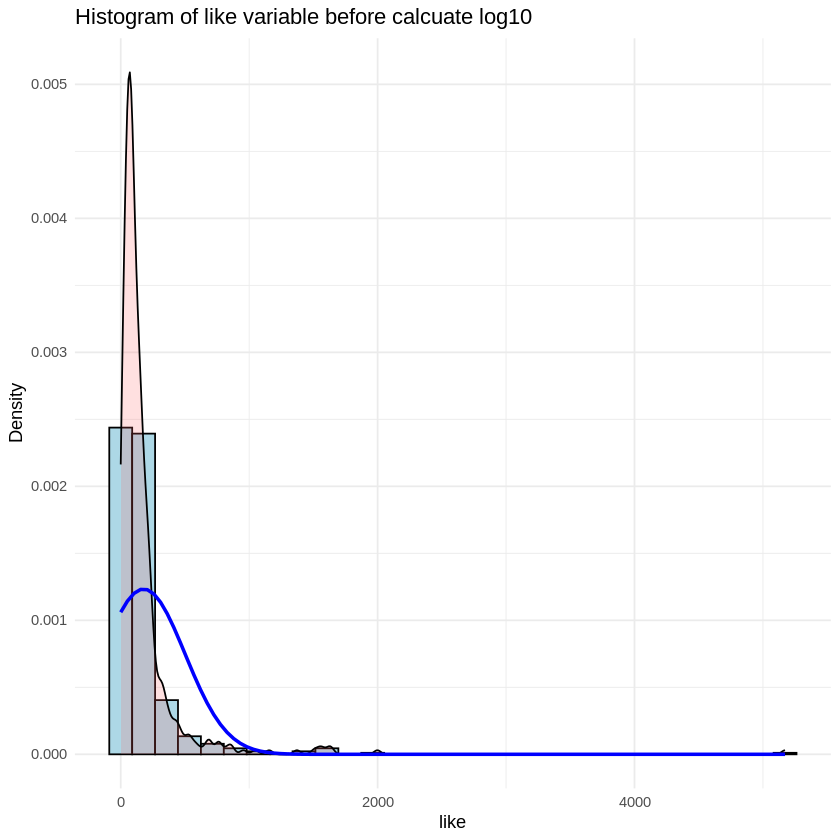
\includegraphics[width=0.8\linewidth]{part01_figures/22.png}
    \caption{Biểu đồ trước khi loại bỏ ngoại lai}
    \label{fig:Biểu đồ trước khi loại bỏ ngoại lai}
\end{figure}
\begin{figure}
    \centering
    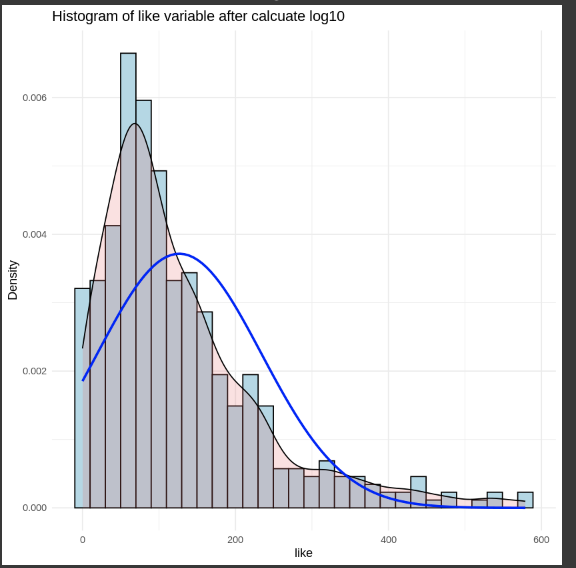
\includegraphics[width=0.8\linewidth]{part23_figures/23.png}
    \caption{Biểu đồ sau khi loại bỏ ngoại lai}
    \label{fig:Biểu đồ sau khi loại bỏ ngoại lai}
\end{figure}
Nhận xét: Sau khi loại bỏ các điểm ngoại lai và cực ngoại lai, ta thu được đồ thị gần chuẩn và có hình dáng tốt hơn trước khi loại.


Tiếp theo chúng ta sẽ tiến hành xây dựng mô hình tương tác và kiểm định các giả thuyết

\begin{lstlisting}
# Shapiro-Wilk test
int_model = aov(like ~ Category * Paid, rm_outliner_data)
summary(int_model)

av_residual = rstandard(int_model)
shapiro.test(av_residual)

# Trực quan bằng QQ plot
qqnorm(av_residual)
qqline(av_residual)
hist(av_residual)
\end{lstlisting}

Kết quả:

\begin{lstlisting}
              Df  Sum Sq Mean Sq F value   Pr(>F)    
Category        2  200989  100494   9.143 0.000129 ***
Paid            1   85534   85534   7.782 0.005512 ** 
Category:Paid   2   11079    5539   0.504 0.604487    
Residuals     430 4726373   10992                     
---
Signif. codes:  0 '***' 0.001 '**' 0.01 '*' 0.05 '.' 0.1 ' ' 1
2 observations deleted due to missingness

	Shapiro-Wilk normality test

data:  av_residual
W = 0.84158, p-value < 2.2e-16
\end{lstlisting}
\begin{figure}
    \centering
    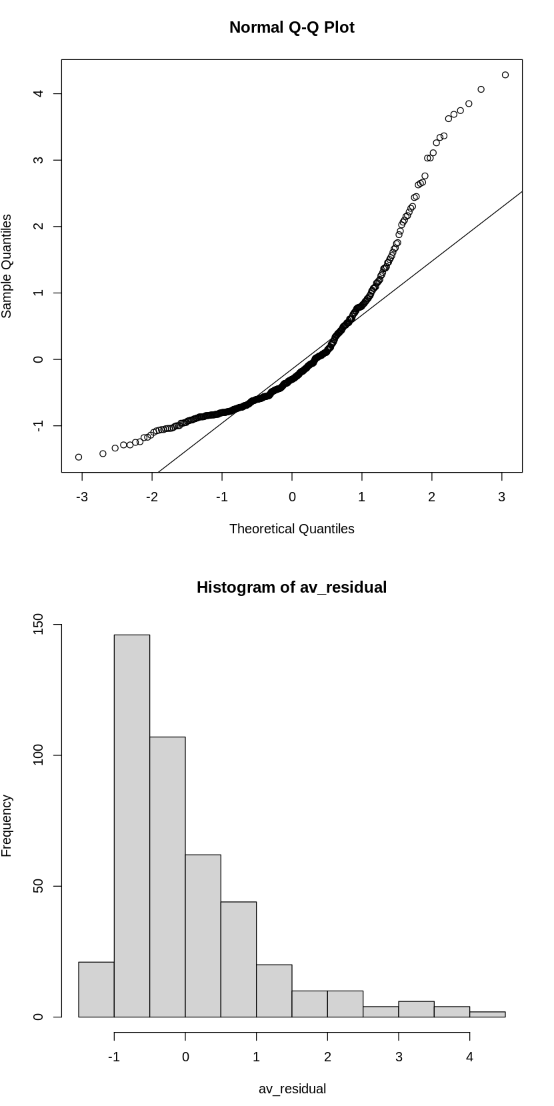
\includegraphics[width=0.5\linewidth]{part23_figures/24.png}
    \caption{Shapiro-Wilk normality test và biểu đồ phần dư}
    \label{fig:Shapiro-Wilk normality test và biểu đồ phần dư}
\end{figure}
Với giả định \begin{itemize}
    \item H0: Phần dư tuân theo phân phối chuẩn
    \item H1: Phần dư không tuân theo phân phối chuẩn
\end{itemize}

Nhận xét: Với mức ý nghĩa 5\%, ta thấy Category vaf Paid có mối liên hệ mật thiết (có tương tác)  tới like. ta thấy rằng phần dư không tuân theo chuẩn nhưng về tổng quan sẽ cho kết quả tốt hơn trước khi chưa xử lý dữ liệu.
\newpage
Tiếp theo chúng ta đi kiểm định tính độc lập của phần dư:
\begin{lstlisting}
# Kiểm định tính độc lập của phần dư
durbinWatsonTest(int_model)
plot(int_model, 1)
\end{lstlisting}
Kết quả
\begin{lstlisting}
lag Autocorrelation D-W Statistic p-value
   1      0.01959622      1.960124   0.678
 Alternative hypothesis: rho != 0
\end{lstlisting}
\begin{figure}[H]
    \centering
    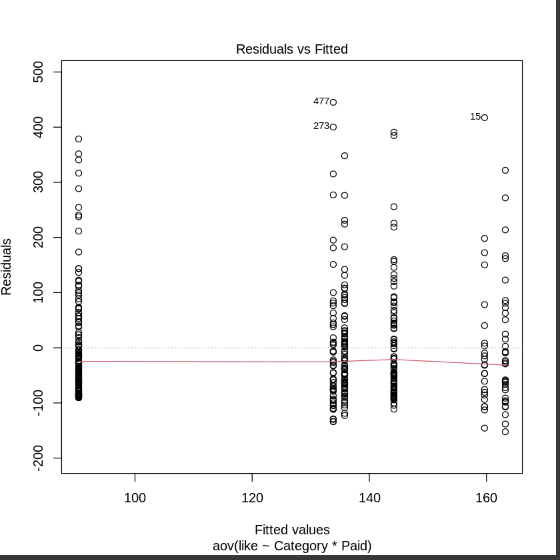
\includegraphics[width=0.5\linewidth]{part23_figures/25.png}
    \caption{Đồ thị  Residuals}
    \label{fig:Đồ thị  Residuals}
\end{figure}

Với mức ý nghĩa 5\%, ta thấy rằng mô hình không có sự tương quan (độc lập)

Tiếp tục Kiểm định các nhóm có phương sai đồng nhất hay không

\begin{lstlisting}
# Kiểm định các nhóm có phương sai đồng nhất hay không
leveneTest(int_model)
\end{lstlisting}

Kết quả
\begin{lstlisting}
A anova: 2 x 3
Df	F value	Pr(>F)
<int>	<dbl>	<dbl>
group	5	0.7839293	0.561649
430	NA	NA

\end{lstlisting}

Với mức ý nghĩa 5\%, ta thấy mô hình có phương sai của các nhóm đồng nhất. Như vậy, ta đủ điều kiện để phân tích ANOVA. Bước tiếp theo, chúng ta sẽ tiến hành kiểm tra tương tác đơn và tương tác chính như phần trước.

% \begin{itemize}
    \item \textbf{Bước 1: Kiểm tra sự tương tác }
    \begin{lstlisting}
summary(int_model)
plot(interactionMeans(int_model))
    \end{lstlisting}

Kết quả:
\begin{figure}[H]
    \centering
    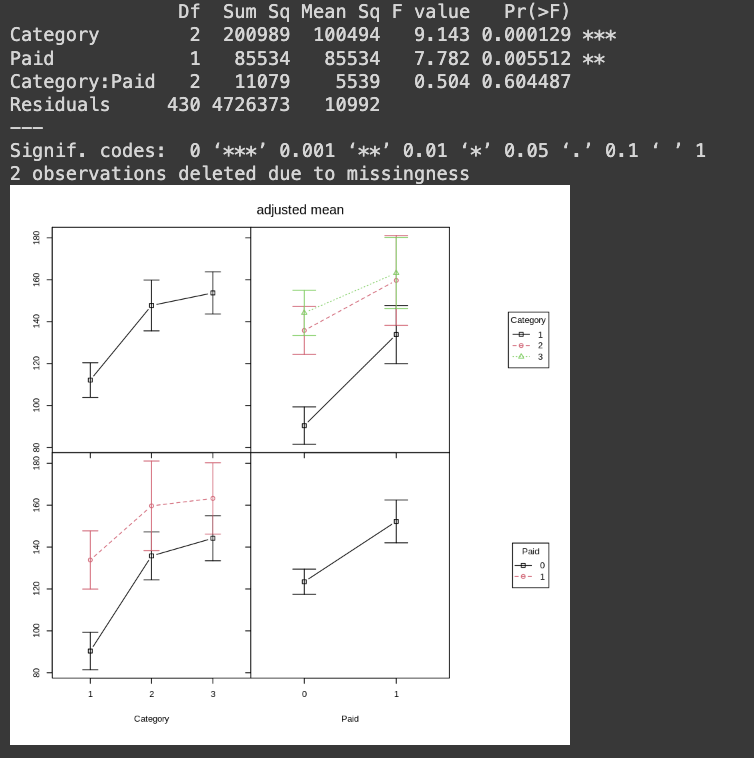
\includegraphics[width=0.8\linewidth]{part23_figures/26.png}
    \caption{Tương tác giữa Category và Paid}
    \label{fig:Tương tác giữa Category và Paid}
\end{figure}

\textbf{Nhận xét:}

    \begin{itemize}
        \item Với mức ý nghĩa 5\% ta thấy giữa \texttt{Category} và \texttt{Paid} không có sự tương tác, nhưng bản thân chúng sẽ có sự ảnh hưởng độc lập đến \texttt{like}. Vì vậy ta chỉ sẽ đi phân tích ảnh hưởng chính của hai thành phần này mà không đi phân tích ảnh hưởng đơn lẻ.
        
        \item \textbf{Biểu đồ bên trái} cho thấy hiệu quả tăng dần khi thay đổi từ 1-2-3 (ảnh hưởng của 3 là rõ rệt nhất trong nhóm \texttt{Category}).
        
        \item \textbf{Biểu đồ bên phải} cho thấy rằng việc sử dụng quảng cáo (\texttt{Paid}) sẽ cho kết quả tốt hơn khi không sử dụng quảng cáo.
    \end{itemize}


   \item \textbf{Bước 3. Phân tích ảnh hưởng chính}
   \begin{itemize}
       \item \textbf{Phân tích ảnh hưởng chính của Category với hiệu quả tương tác bài post thông qua lượt like}
       \begin{lstlisting}
category_model = lm(like~Category, data = rm_outliner_data)
summary(category_model)
       \end{lstlisting}
       Kết quả:
       \begin{lstlisting}
             Call:
lm(formula = like ~ Category, data = rm_outliner_data)

Residuals:
    Min      1Q  Median      3Q     Max 
-138.63  -73.09  -31.09   39.91  475.91 

Coefficients:
            Estimate Std. Error t value Pr(>|t|)    
(Intercept)  103.092      7.551  13.653  < 2e-16 ***
Category2     37.541     12.610   2.977 0.003074 ** 
Category3     46.539     11.858   3.925 0.000101 ***
---
Signif. codes:  0 '***' 0.001 '**' 0.01 '*' 0.05 '.' 0.1 ' ' 1

Residual standard error: 105.4 on 434 degrees of freedom
  (1 observation deleted due to missingness)
Multiple R-squared:  0.03975,	Adjusted R-squared:  0.03533 
F-statistic: 8.984 on 2 and 434 DF,  p-value: 0.0001503            
       \end{lstlisting}
    Nhận xét: Nhận xét: Với mức ý nghĩa 0.05, ta thấy rằng các nhóm category đều ảnh hưởng đến số lượt like
    \begin{lstlisting}
# Shapiro-Wilk test
av_residual = rstandard(category_model)
shapiro.test(av_residual)

# Trực quan bằng QQ plot
qqnorm(av_residual)
qqline(av_residual)
hist(av_residual)
    \end{lstlisting}
    Kết quả:
    \begin{lstlisting}
	Shapiro-Wilk normality test

data:  av_residual
W = 0.83235, p-value < 2.2e-16
    \end{lstlisting}
    \begin{figure}[H]
        \centering
        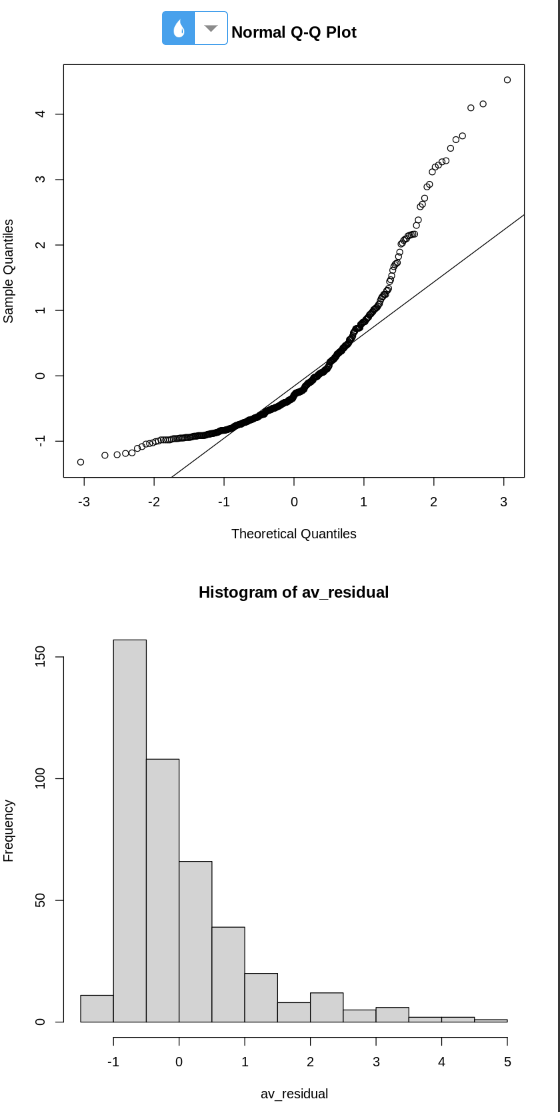
\includegraphics[width=0.8\linewidth]{part23_figures/27.png}
        \caption{Shapiro-test}
        \label{fig:Shapiro-test và đồ thị phân phối}
    \end{figure}

    Nhận xét: Giá trị p-value đã tăng lên rất nhiều (mặc dù < 0.05), hình dáng đồ thị gần chuẩn hơn so với trước khi chưa xử lý dữ liệu
   \end{itemize}
    \begin{lstlisting}
# Kiểm định các nhóm có phương sai đồng nhất hay không
leveneTest(category_model)
    \end{lstlisting}
    Kết quả:
    \begin{lstlisting}
A anova: 2 x 3
Df	F value	Pr(>F)
<int>	<dbl>	<dbl>
group	2	0.1707522	0.843087
434	NA	NA

    \end{lstlisting}
    Nhận xét:
    Với các giả định:
        \begin{itemize}
            \item H0: Các nhóm có phương sai đồng nhất
            \item H1: Các nhóm không có phương sai đồng nhất
        \end{itemize}
    Nhận xét: Với giá trị p-value = 0.843087 > 0.05, ta không điều kiện bác bỏ H0, vậy các nhóm có phương sai đồng nhất (giá trị p-value tăng lên).
    \begin{lstlisting}
# Kiểm định tính độc lập của phần dư
durbinWatsonTest(category_model)
plot(category_model, 1)
    \end{lstlisting}
    Kết quả:
    \begin{figure}[H]
        \centering
        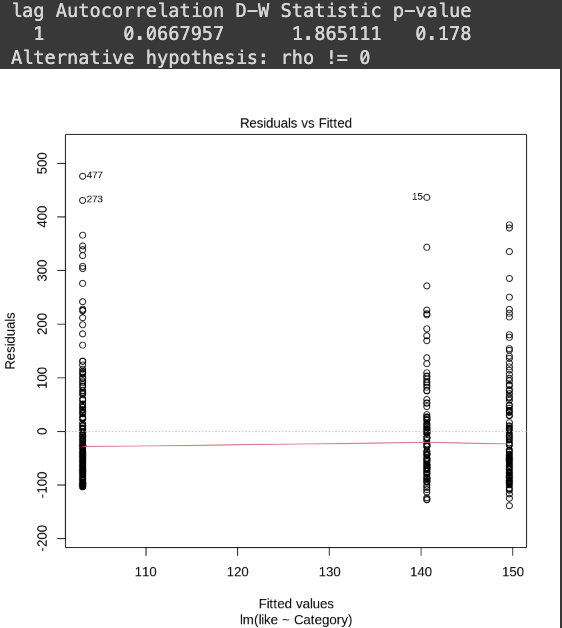
\includegraphics[width=0.8\linewidth]{part23_figures/28.png}
        \caption{Kiểm định độc lập phần dư}
        \label{fig:Kiểm định độc lập phần dư__}
    \end{figure}

        Nhận xét:
    Với các giả định:
        \begin{itemize}
            \item H0: Không có sự tương quan (độc lập)
            \item H1: Có sự tương quan (không độc lập)
        \end{itemize}
    Nhận xét:Với giá trị p-value = 0.178 nên có sự tương quan dương, tuy nhiên kết quả này lớn hơn kết quả trước đó (=0).
    \begin{lstlisting}
# Kiểm định trung bình giữa các nhóm 
with(rm_outliner_data, pairwise.t.test(like, Category, p.adj = "bonferroni"))
TukeyHSD(aov(like~Category, data=rm_outliner_data), conf.level = 0.95)
plot(TukeyHSD(aov(like~Category, data=rm_outliner_data), conf.level = 0.95))
    \end{lstlisting}
    Kết quả:
    \begin{figure}[H]
        \centering
        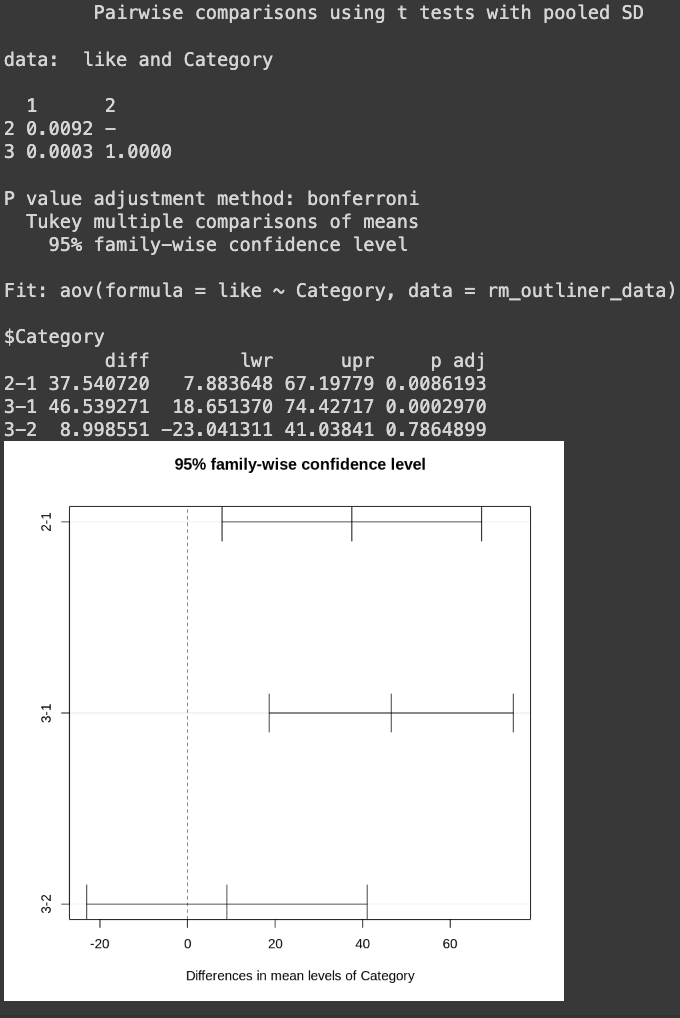
\includegraphics[width=0.8\linewidth]{part23_figures/29.png}
        \caption{Kiểm định trung bình}
        \label{fig:Kiểm định trung bình}
    \end{figure}

    Với các giả định:
        \begin{itemize}
            \item H0: Các giá trị trung bình giữa các cặp bằng nhau
            \item H1: Các giá trị trung bình giữa các cặp không bằng nhau
        \end{itemize}
    Nhận xét: \begin{itemize}
        \item Cặp 2-1 và 3-1 không có mean bằng nhau (đồ thị ko cắt điểm 0, p-value > 0.05)
        \item Cặp 3-2 có mean bằng nhau (đồ thị cắt điểm 0, p-value < 0.05)
    \end{itemize}

    \item \textbf{Phân tích ảnh hưởng chính của Quảng cáo với hiệu quả của bài post thông qua số lượt like}
    \begin{lstlisting}
paid_model = lm(like~Paid, data = rm_outliner_data)
summary(paid_model)
    \end{lstlisting}
    Kết quả:
    \begin{lstlisting}
             Call:
lm(formula = like ~ Paid, data = rm_outliner_data)

Residuals:
    Min      1Q  Median      3Q     Max 
-148.43  -71.43  -29.55   40.70  430.57 

Coefficients:
            Estimate Std. Error t value Pr(>|t|)    
(Intercept)  118.546      5.996  19.770  < 2e-16 ***
Paid1         29.883     11.478   2.604  0.00954 ** 
---
Signif. codes:  0 '***' 0.001 '**' 0.01 '*' 0.05 '.' 0.1 ' ' 1

Residual standard error: 106.8 on 434 degrees of freedom
  (2 observations deleted due to missingness)
Multiple R-squared:  0.01538,	Adjusted R-squared:  0.01311 
F-statistic: 6.779 on 1 and 434 DF,  p-value: 0.009542
    \end{lstlisting}
    Nhận xét: Với mức ý nghĩa 0.05, ta thấy rằng Paid có ý nghĩa trong việc giải thích mô hình.
    \begin{lstlisting}
# Shapiro-Wilk test
av_residual = rstandard(paid_model)
shapiro.test(av_residual)

# Trực quan bằng QQ plot
qqnorm(av_residual)
qqline(av_residual)
hist(av_residual)
    \end{lstlisting}

    Kết quả:
    \begin{lstlisting}
	Shapiro-Wilk normality test

data:  av_residual
W = 0.9859, p-value = 0.07921
    \end{lstlisting}
\begin{figure}
    \centering
    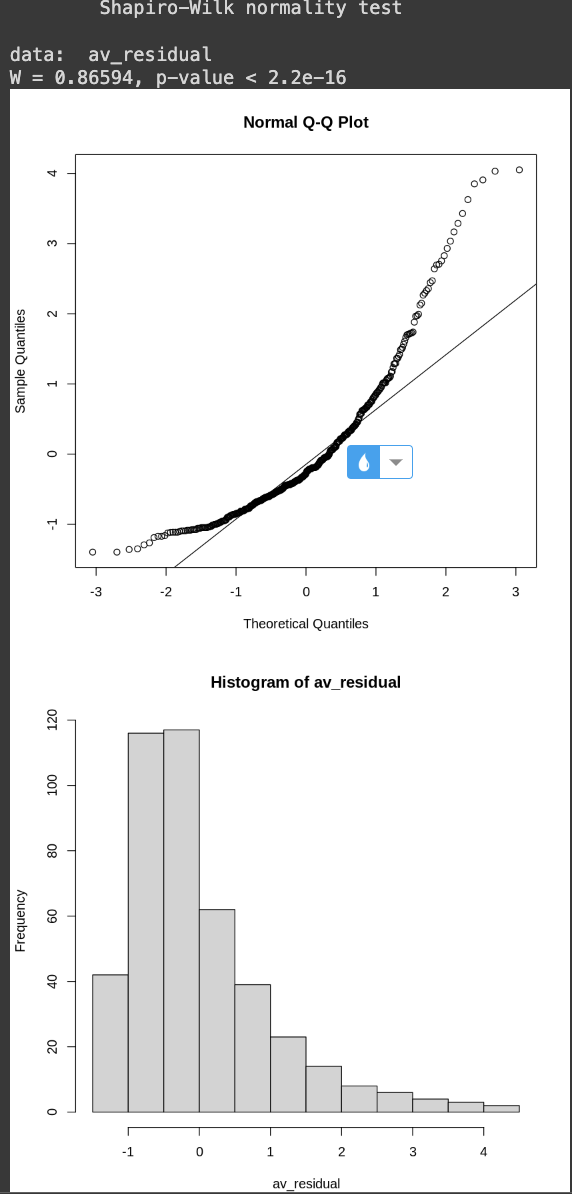
\includegraphics[width=0.5\linewidth]{part23_figures/30.png}
    \caption{Shapiro-Wilk normality test và độ thị phân phối}
    \label{fig:Shapiro-Wilk normality test và đồ thị phân phối}
\end{figure}

    Với các giả định:
    \begin{itemize}
        \item H0: Tuân theo phân phối chuẩn
        \item H1: Không tuân theo phân phối chuẩn
    \end{itemize}
    Nhận xét: với độ tin cậy 5\% thì với giá trị p-value = 2.2e-16 chúng ta đủ cơ sở bác bỏ H0, vậy sai số có phân phối không chuẩn. (Giống kết quả trước đó), tuy nhiên về biểu đồ phân phối cho ta kết quả đẹp hơn

    \begin{lstlisting}
# Kiểm định các nhóm có phương sai đồng nhất hay không
leveneTest(drug_model)
    \end{lstlisting}
    Kết quả:
    \begin{lstlisting}
A anova: 2 x 3
Df	F value	Pr(>F)
<int>	<dbl>	<dbl>
group	1	2.750614	0.09793961
434	NA	NA

    \end{lstlisting}
    Với các giả định:
    \begin{itemize}
        \item H0: Các nhóm có phương sai đồng nhất
        \item H1: Các nhóm không có phương sai đồng nhất
    \end{itemize}
    Nhận xét: Với giá trị p-value = 0.097 > 0.05, ta không đủ điều kiện bác bỏ H0, vậy các nhóm có phương sai đồng nhất (giống cũ)
\begin{lstlisting}
# Kiểm định tính độc lập của phần dư
durbinWatsonTest(paid_model)
plot(paid_model, 1)
\end{lstlisting}
\begin{figure}[H]
    \centering
    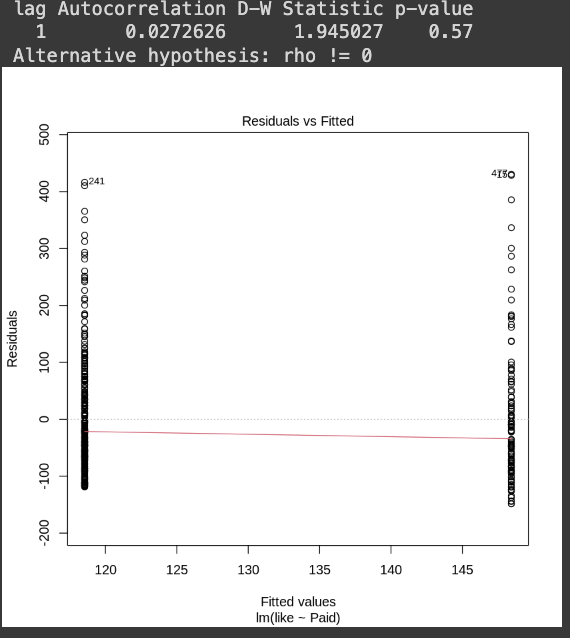
\includegraphics[width=0.8\linewidth]{part23_figures/31.png}
    \caption{Kiểm định tính độc lập của phần dư}
    \label{fig:Kiểm định tính độc lập của phần dư_}
\end{figure}
    Với các giả định:
    \begin{itemize}
        \item H0: Không có sự tương quan (độc lập)
        \item H1: Có sự tương quan (không độc lập)
    \end{itemize}
    Nhận xét: Với giá trị p-value = 0.57 nên không có sự tương quan (trước đó là 0.11).

\begin{lstlisting}
# Kiểm định độ hiệu quả trung bình
with(rm_outliner_data, pairwise.t.test(like, Paid, p.adj = "bonferroni"))
TukeyHSD(aov(like~Paid, data=rm_outliner_data), conf.level = 0.95)
plot(TukeyHSD(aov(like~Paid, data=rm_outliner_data), conf.level = 0.95))

\end{lstlisting}
\begin{figure}[H]
    \centering
    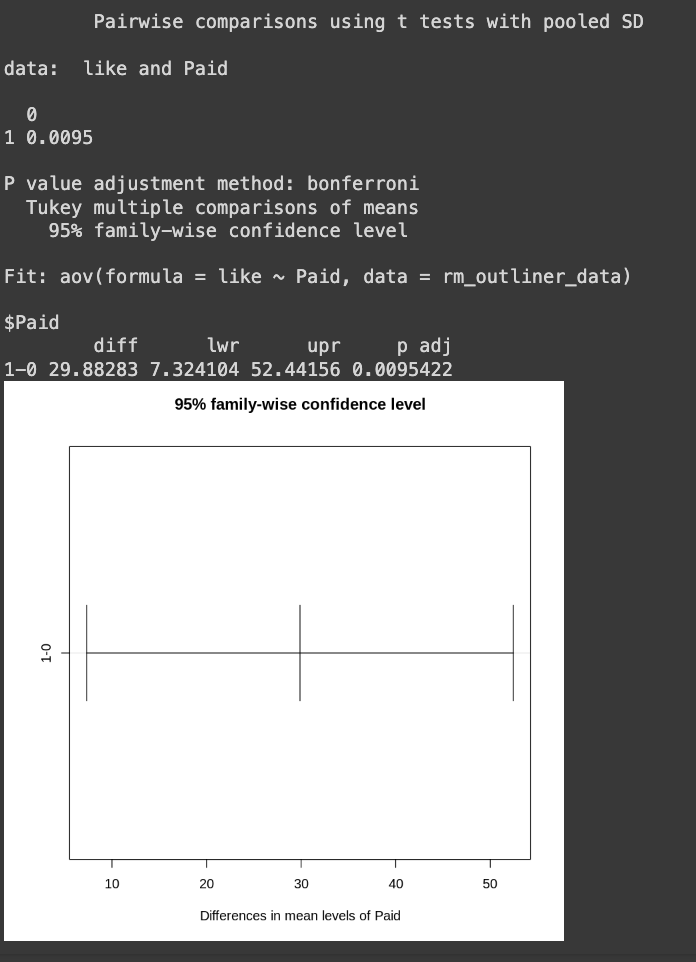
\includegraphics[width=0.8\linewidth]{part23_figures/32.png}
    \caption{Kiểm định độ hiệu quả trung bình}
    \label{fig:Kiểm định độ hiệu quả trung bình}
\end{figure}
    Với các giả định:
    \begin{itemize}
        \item H0: Các giá trị trung bình giữa các cặp bằng nhau
        \item H1: Các giá trị trung bình giữa các cặp không bằng nhau
    \end{itemize}
    Nhận xét: Nhìn vào kết quả ta có: Với p-value = 0.095 thì ta không đủ điều kiện bác bỏ H0, vậy 2 nhóm có mean bằng nhau.
    
    \item \textbf{Bước 4: Xây dựng và kiểm định mô hình cộng (Additive model)}
    \begin{lstlisting}
add_model = lm(like~., data=rm_outliner_data)
add_model <- MASS::stepAIC(add_model, k = log(nrow(rm_outliner_data)), trace = 0)
summary(add_model)
add_model$coefficients
    \end{lstlisting}
    Kết quả:
    \begin{lstlisting}

Call:
lm(formula = like ~ Category + Paid, data = rm_outliner_data)

Residuals:
    Min      1Q  Median      3Q     Max 
-161.14  -71.10  -32.51   44.18  453.61 

Coefficients:
            Estimate Std. Error t value Pr(>|t|)    
(Intercept)   93.882      8.192  11.460  < 2e-16 ***
Category2     40.209     12.586   3.195  0.00150 ** 
Category3     46.747     11.777   3.969 8.44e-05 ***
Paid1         31.510     11.283   2.793  0.00546 ** 
---
Signif. codes:  0 '***' 0.001 '**' 0.01 '*' 0.05 '.' 0.1 ' ' 1

Residual standard error: 104.7 on 432 degrees of freedom
  (2 observations deleted due to missingness)
Multiple R-squared:  0.05703,	Adjusted R-squared:  0.05048 
F-statistic: 8.709 on 3 and 432 DF,  p-value: 1.275e-05
(Intercept)93.8817153094315
Category240.2086725476412
Category346.7470289779827
Paid131.5099213098397

    \end{lstlisting}
   Nhận xét: Với p-value=5\%, cả 2 biến đều có ý nghĩ trong việc giải thích mô hình. Ta tiến hành kiểm định Shapiro và Breusch-Pagan

\begin{lstlisting}
# Shapiro-Wilk test
av_residual = rstandard(add_model)
shapiro.test(av_residual)

# Trực quan bằng QQ plot
qqnorm(av_residual)
qqline(av_residual)
hist(av_residual)
\end{lstlisting}

\begin{figure}[H]
    \centering
    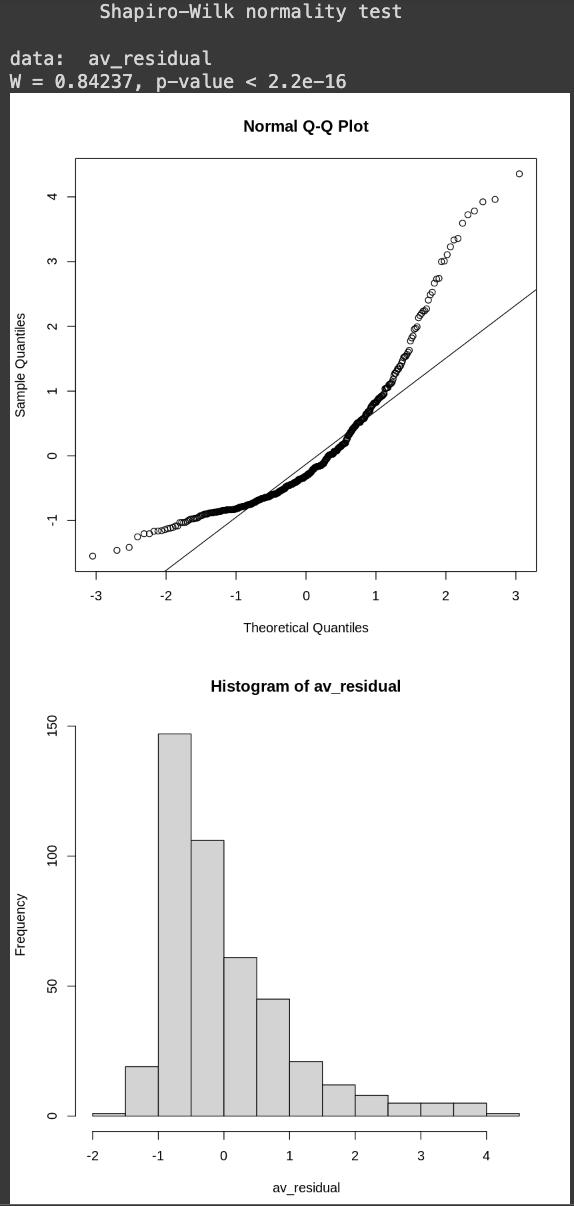
\includegraphics[width=0.8\linewidth]{part23_figures/33.png}
    \caption{Shapiro test và biểu đồ phân phối}
    \label{fig:Shapiro test và biểu đồ phân phối}
\end{figure}

Nhận xét: với độ tin cậy 5\% thì với giá trị p-value = 2.2e-16 chúng ta đủ cơ sở bác H0, vậy phần dư không tuân theo chuẩn (giống trước).

\begin{lstlisting}
    # Kiểm định tính độc lập của phần dư
durbinWatsonTest(add_model)
plot(add_model, 1)
\end{lstlisting}

Kết quả:
\begin{lstlisting}
    lag Autocorrelation D-W Statistic p-value
   1      0.02458993      1.950179   0.606
 Alternative hypothesis: rho != 0
\end{lstlisting}


Nhận xét: Với giá trị p-value = 0.606 nên có sự tương quan dương, tuy nhiên kết quả tốt hơn trước (0.412).

\begin{lstlisting}
# Kiểm định  Breusch-Pagan
bptest(add_model)
add_model$coefficients
\end{lstlisting}
Kết quả:
\begin{lstlisting}
    studentized Breusch-Pagan test

data:  add_model
BP = 4.3594, df = 3, p-value = 0.2252
(Intercept)93.8817153094315 Category240.2086725476412   Category346.7470289779827
Paid131.5099213098397
\end{lstlisting}
 Với p-value=0.2252 > 0.05 thì ta không đủ điều kiện bác bỏ H0. Vậy phương sai của mô hình độc lập.
Như vậy, mô hình cộng được xây dựng như sau:

\textbf{Mô hình cộng được xây dựng như sau:}

\begin{equation}
\texttt{like} = 93.38 + 40.20 \times \texttt{Category2} + 46.747 \times \texttt{Category3} + 31.51 \times \texttt{Paid1}
\end{equation}

\begin{itemize}
    \item \textbf{Category2 (40.21)}: Khi biến \texttt{Category} chuyển từ mức cơ bản (\texttt{Category1}) sang \texttt{Category2}, biến phụ thuộc tăng trung bình 40.21 đơn vị.
    \item \textbf{Category3 (46.75)}: Khi biến \texttt{Category} chuyển từ mức cơ bản (\texttt{Category1}) sang \texttt{Category3}, biến phụ thuộc tăng trung bình 46.75 đơn vị.
    \item \textbf{Paid1 (31.51)}: Khi biến \texttt{Paid} chuyển từ mức cơ bản (\texttt{Paid0}) sang \texttt{Paid1}, biến phụ thuộc tăng trung bình 31.51 đơn vị.
\end{itemize}

\textbf{Kết luận:} Như vậy để tăng tương tác bài viết, người dùng có thể sử dụng quảng cáo và nội dung liên quan đến chủ đề 2 và 3 (chủ đề 3 cho kết quả cao hơn).

\textbf{Nhận xét chung:} Như vậy về tổng thể, sau khi loại bỏ các điểm ngoại lai và cực ngoại lai, việc thống kê và phân tích ANOVA đã cho ra một mô hình có các yếu tố thỏa mãn các kiểm định về chuẩn hơn. Trong trường hợp không chuẩn, các chỉ số đã được cải thiện so với trước đây.

\end{itemize}
